\documentclass{article}

\usepackage[preprint]{neurips}

\makeatletter
\renewcommand{\@notice}{}
\makeatother

\usepackage[utf8]{inputenc}
\usepackage[T1]{fontenc}
\usepackage{amsmath}
\usepackage{amssymb}
\usepackage{booktabs}
\usepackage{array}
\usepackage{graphicx}
\usepackage{adjustbox}
\usepackage{caption}
\usepackage{subcaption}
\usepackage{float}
\usepackage{placeins}
\usepackage{xcolor}
\usepackage{hyperref}
\usepackage{url}
\usepackage{tikz}
\usetikzlibrary{arrows.meta,positioning,fit}

\hypersetup{
  colorlinks=true,
  linkcolor=blue,
  citecolor=blue,
  urlcolor=blue
}

\raggedbottom
\setlength{\textfloatsep}{7pt plus 2pt minus 2pt}
\setlength{\intextsep}{7pt plus 2pt minus 2pt}
\setlength{\floatsep}{6pt plus 2pt minus 2pt}
\renewcommand{\topfraction}{0.97}
\renewcommand{\bottomfraction}{0.90}
\renewcommand{\textfraction}{0.03}
\renewcommand{\floatpagefraction}{0.88}
\setcounter{topnumber}{5}
\setcounter{bottomnumber}{4}
\setcounter{totalnumber}{9}
\captionsetup{font=small,skip=3pt}

\newcommand{\pct}{\%\ }
\newcommand{\Efive}{\ensuremath{E^{(5)}}}
\newcommand{\Etwo}{\ensuremath{E^{(2)}}}
\newcommand{\CM}{\ensuremath{C_M}}
\newcommand{\CR}{\ensuremath{C_R}}
\newcommand{\EM}{\ensuremath{E_M}}
\newcommand{\ER}{\ensuremath{E_R}}

\title{Assignment 2 Report: River Forecasting and Robust Motion Prediction}

\author{
  Daniyal Hussain Shah
}

\begin{document}

\maketitle

\begin{abstract}
This report studies two forecasting problems in which useful predictions require the right information to travel through the model. Question 1 proposes a delay-aware spatio-temporal graph forecaster for one-hour river-level prediction at four stations. The design uses only information available at issuance, represents directed river connectivity and distance, incorporates announced releases as known future inputs, and produces calibrated uncertainty intervals. Question 2 tests whether a ConvLSTM learns motion or only familiar Moving MNIST appearances and speeds. Model A is accurate at normal speed but is not exactly consistent under mirror or rotation and degrades sharply at faster motion. Symmetry augmentation reduces consistency gaps, while speed augmentation produces the largest fast-motion improvement. Model D extends nominal reach from 8 to 16 pixels and records a smaller additional 3x gain, but its dilation also creates disconnected parity lattices, so the gain is not a clean reach-only effect. Wrapping D in an eight-way symmetrised forecaster makes mirror and rotation consistency exact up to floating-point error, but increases inference cost and does not remove forecast blur. Code, notebooks, GIFs, and machine-readable results are available at \url{https://github.com/syeddaniyalg/cs434-pa2}.
\end{abstract}

\section{Introduction}

Forecasting quality depends on whether the model receives the relevant causes and whether its architecture can connect them to the prediction. A river forecast can fail because an upstream release, tributary inflow, or delayed observation is missing or misaligned. A video forecast can fail even with complete frames because the learned rule is tied to familiar digit appearance, unfamiliar speed, or a spatial reach that is too short for the displacement.

Question 1 treats these issues as a system-design problem. It specifies a causal issuance-time data pipeline, a directed river graph, a delay-aware spatio-temporal model, operational handling of imperfect observations, and uncertainty outputs. Question 2 separates appearance, motion exposure, and architectural reach through controlled Moving MNIST experiments. Every learned model is evaluated for two seeds, and every consistency gap is reported with the corresponding transformed error.

\section*{Question 1: River Forecasting Proposal}
\label{sec:q1}

\subsection*{1. Architecture diagram}

The architecture diagram below shows the proposed service. Historical measurements are aligned to a ten-minute grid, with masks and observation ages retained. Rainfall is projected from two gauges to five observed hydrological nodes. Realised releases and the schedule known at issuance are attached only to S1, where reservoir water enters the monitored river. A latent tributary state enters between S2 and S3 and is inferred from rainfall and historical routing residuals. A causal encoder is followed by a six-step forecast rollout with three directed graph blocks per step, enough for information to traverse S1--S2--S3--S4. The decoder returns the one-hour-ahead median and prediction interval for S1--S4.

\begin{figure}[htbp]
\centering
\resizebox{\linewidth}{!}{
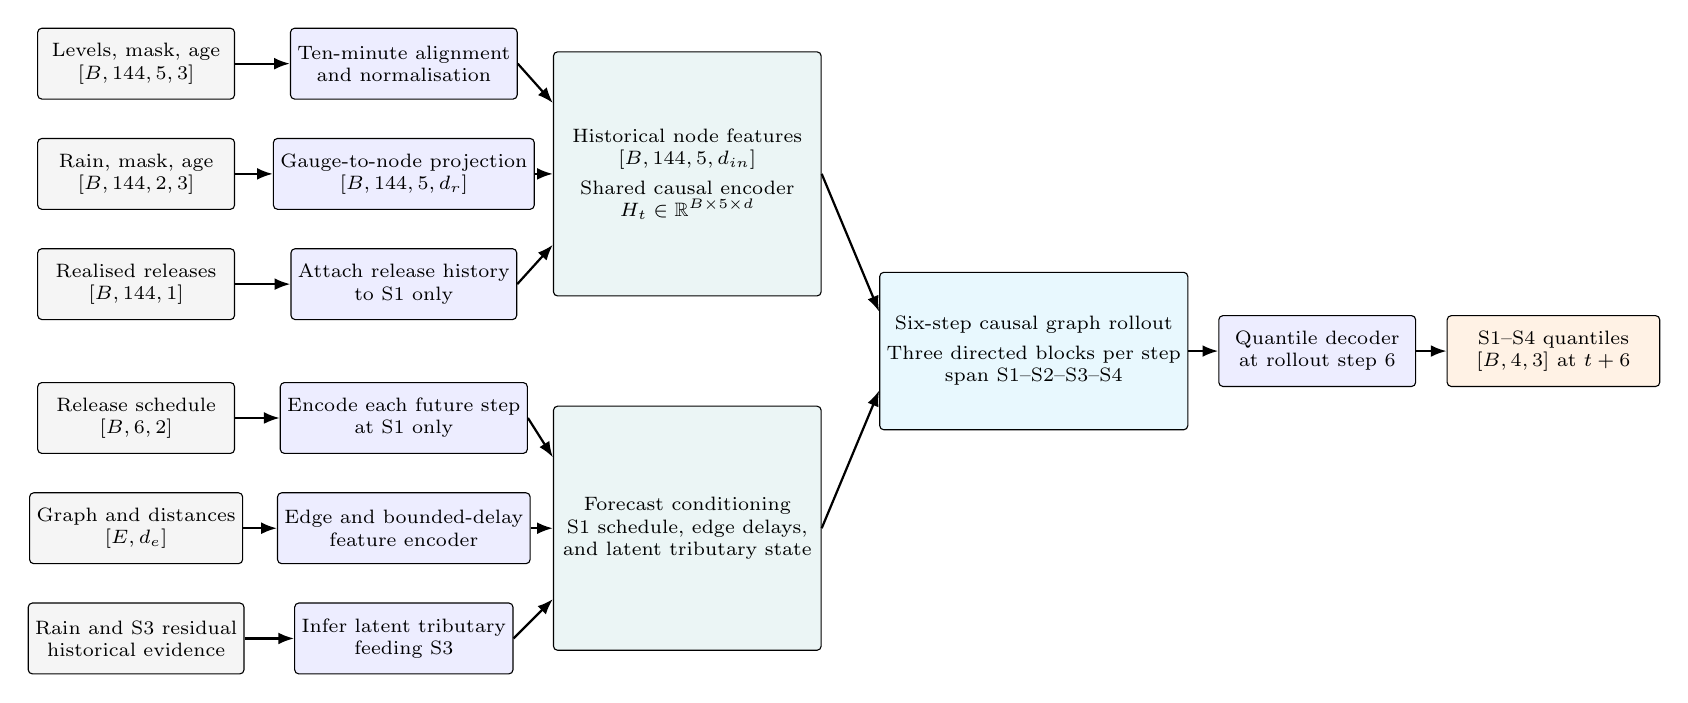
\begin{tikzpicture}[
  box/.style={draw, rounded corners=1.5pt, align=center, minimum height=9mm, minimum width=25mm, inner sep=2.5pt, font=\scriptsize},
  source/.style={box, fill=gray!8},
  transform/.style={box, fill=blue!7},
  group/.style={box, fill=teal!8, minimum width=34mm, minimum height=31mm},
  rollout/.style={box, fill=cyan!9, minimum width=38mm, minimum height=20mm},
  output/.style={box, fill=orange!10, minimum width=27mm},
  arrow/.style={-{Latex[length=2mm]}, thick}
]
\node[source] (levels) at (0,3.0) {Levels, mask, age\\$[B,144,5,3]$};
\node[source] (rain) at (0,1.6) {Rain, mask, age\\$[B,144,2,3]$};
\node[source] (releasehist) at (0,0.2) {Realised releases\\$[B,144,1]$};
\node[source] (schedule) at (0,-1.5) {Release schedule\\$[B,6,2]$};
\node[source] (static) at (0,-2.9) {Graph and distances\\$[E,d_e]$};
\node[source] (residual) at (0,-4.3) {Rain and S3 residual\\historical evidence};

\node[transform] (align) at (3.4,3.0) {Ten-minute alignment\\and normalisation};
\node[transform] (rainproj) at (3.4,1.6) {Gauge-to-node projection\\$[B,144,5,d_r]$};
\node[transform] (releaseenc) at (3.4,0.2) {Attach release history\\to S1 only};
\node[transform] (scheduleenc) at (3.4,-1.5) {Encode each future step\\at S1 only};
\node[transform] (edge) at (3.4,-2.9) {Edge and bounded-delay\\feature encoder};
\node[transform] (latent) at (3.4,-4.3) {Infer latent tributary\\feeding S3};

\node[group] (history) at (7.0,1.6) {Historical node features\\$[B,144,5,d_{in}]$\\[1mm]Shared causal encoder\\$H_t\in\mathbb{R}^{B\times5\times d}$};
\node[group] (conditioning) at (7.0,-2.9) {Forecast conditioning\\S1 schedule, edge delays,\\and latent tributary state};
\node[rollout] (forecast) at (11.4,-0.65) {Six-step causal graph rollout\\[1mm]Three directed blocks per step\\span S1--S2--S3--S4};
\node[transform] (decoder) at (15.0,-0.65) {Quantile decoder\\at rollout step 6};
\node[output] (out) at (18.0,-0.65) {S1--S4 quantiles\\$[B,4,3]$ at $t+6$};

\draw[arrow] (levels) -- (align);
\draw[arrow] (rain) -- (rainproj);
\draw[arrow] (releasehist) -- (releaseenc);
\draw[arrow] (schedule) -- (scheduleenc);
\draw[arrow] (static) -- (edge);
\draw[arrow] (residual) -- (latent);

\draw[arrow] (align.east) -- ([yshift=9mm]history.west);
\draw[arrow] (rainproj.east) -- (history.west);
\draw[arrow] (releaseenc.east) -- ([yshift=-9mm]history.west);
\draw[arrow] (scheduleenc.east) -- ([yshift=9mm]conditioning.west);
\draw[arrow] (edge.east) -- (conditioning.west);
\draw[arrow] (latent.east) -- ([yshift=-9mm]conditioning.west);

\draw[arrow] (history.east) -- ([yshift=5mm]forecast.west);
\draw[arrow] (conditioning.east) -- ([yshift=-5mm]forecast.west);
\draw[arrow] (forecast) -- (decoder);
\draw[arrow] (decoder) -- (out);
\end{tikzpicture}
}
\caption*{River forecasting architecture. Five observed nodes represent S1--S4 and T1; the unmonitored tributary is a latent node feeding S3. Historical encoding and future conditioning remain separate until the causal rollout.}
\end{figure}

\subsection*{2. Assumptions}

The supplied facts are the ten-minute sampling interval, observed stations S1--S4 and T1, gauges R1--R2, the directed river connectivity and distances, announced future releases, and the one-hour target at S1--S4. The following are assumptions required to turn those facts into an operational design.

\paragraph{A1. Ten-minute alignment is feasible.}
Water-level, rainfall, and release records can be converted to one time zone and aligned to the station clock. Off-grid observations are assigned only to intervals in which they were available; no future value is used.

\paragraph{A2. Record length is adequate.}
At least one year of data is available and contains ordinary flow, rainfall events, reservoir changes, and several high-water episodes. If extreme events are rare, uncertainty estimates will be wider and evaluation will be stratified by water-level regime.

\paragraph{A3. Measurements are calibrated.}
Station datum changes and sensor replacements are documented. Undocumented shifts would be confused with hydrological change, so detected level shifts are flagged rather than silently normalised.

\paragraph{A4. Flow is mainly directed downstream.}
The supplied connectivity determines message direction. Local autoregressive state remains available at every node, allowing the model to represent persistence and some backwater effects without inventing reverse river edges.

\paragraph{A5. Distance constrains influence but not fixed travel time.}
Longer river distance generally implies a longer delay, but the delay changes with level and recent flow. Distance is therefore a static edge feature, while effective delay is learned from recent conditions.

\paragraph{A6. Rain gauges are informative but spatially incomplete.}
R1 and R2 are treated as noisy observations of basin rainfall. Their location-aware projections may be uncertain for ungauged sub-catchments.

\paragraph{A7. Release schedules are versioned.}
Every announcement has an issue time and effective time. At issuance, the model uses only the latest schedule announced by that time. Later revisions cannot enter an earlier forecast.

\paragraph{A8. Reporting latency is observable and usually below ten minutes.}
Each value retains event and arrival time. Values arriving after the next forecast cycle are treated as missing for that issuance, so the service still operates but widens its interval and raises a degraded-data flag.

\subsection*{3. Forecasting task and data specification}

A forecast is issued immediately after the ten-minute observation at time $t$ has been processed. The history length is 24 hours, so $L=144$. The target is the four-vector of station levels at $t+6$, one hour after issuance. Training examples are indexed by issue time and never use measurements or announcements that became available later.

\begin{table}[htbp]
\centering
\caption*{River forecasting data specification. $B$ is batch size, $L=144$, $F=6$, $N_w=5$ water-level nodes, $N_r=2$ rain gauges, and $Q=3$ quantiles.}
\footnotesize
\begin{adjustbox}{max width=\linewidth}
\begin{tabular}{llll}
\toprule
Variable & Tensor shape & Axes & Time coverage / availability \\
\midrule
Water levels S1--S4, T1 & $[B,L,N_w,1]$ & batch, time, node, value & $t-143,\ldots,t$ \\
Water mask and age & $[B,L,N_w,2]$ & batch, time, node, feature & Known at issuance \\
Rainfall R1--R2 & $[B,L,N_r,1]$ & batch, time, gauge, value & $t-143,\ldots,t$ \\
Rain mask and age & $[B,L,N_r,2]$ & batch, time, gauge, feature & Known at issuance \\
Realised releases & $[B,L,1]$ & batch, time, release & $t-143,\ldots,t$ \\
Announced releases & $[B,F,2]$ & batch, future time, amount/mask & Effective at $t+1,\ldots,t+6$ and announced by $t$ \\
Node locations/types & $[N_w,d_n]$ & node, static feature & Static \\
Directed edges/distances & $[E,d_e]$ & edge, static feature & Static \\
Forecast quantiles & $[B,4,Q]$ & batch, target station, quantile & Levels at $t+6$ \\
\bottomrule
\end{tabular}
\end{adjustbox}
\end{table}

Values are normalised with training-only statistics, separately by variable and station. Missing values are temporarily filled after normalisation, but the mask and time since last valid observation are always supplied. Rainfall is projected to hydrological nodes with weights conditioned on gauge-node distance and learned location embeddings. Timestamps remain explicit during alignment so a delayed report is not treated as contemporaneous.

\subsection*{4. Model computations and design justification}

Let $x_{i,s}$ be the dynamic feature vector for hydrological node $i$ at time $s$. A shared causal temporal encoder produces
\begin{equation}
  h_{i,s}=\operatorname{GRU}_{\theta}\!\left(x_{i,s},h_{i,s-1}\right).
\end{equation}
Sharing $\theta$ prevents each station from becoming an unrelated forecasting problem. Station identity, location, and node type are included as embeddings, so shared dynamics can still have location-specific effects.

Forecasting is an explicit causal rollout. Let $\tilde h_{i,t}=h_{i,t}$ and let $k\in\{1,\ldots,6\}$ index the future ten-minute steps. For a directed edge $j\rightarrow i$, the state relevant at target step $k$ is
\begin{equation}
  u_{ji,k}=t+k-\delta_{ji,k},\qquad
  \bar h_{j,u_{ji,k}}=
  \begin{cases}
    h_{j,u_{ji,k}}, & u_{ji,k}\leq t,\\
    \tilde h_{j,u_{ji,k}}, & u_{ji,k}>t,
  \end{cases}
\end{equation}
using linear interpolation between adjacent states for a non-integer delay. Thus water arriving at $t+6$ uses upstream state at $t+6-\delta$, not state at $t-\delta$. If the travel time is shorter than the forecast horizon, the unavailable portion comes from earlier forecast states rather than future observations. The delay is constrained by distance and recent flow. Each rollout step applies three message-passing blocks,
\begin{align}
  m_{i,k}^{(\ell)}
  &=\sum_{j\in\mathcal{N}^{-}(i)}
  \alpha_{ji,k}^{(\ell)}W_{\phi}^{(\ell)}
  [\bar h_{j,u_{ji,k}}^{(\ell)};e_{ji}],\\
  \tilde h_{i,t+k}^{(\ell+1)}
  &=\operatorname{LayerNorm}\!\left(\tilde h_{i,t+k}^{(\ell)}+
  \operatorname{MLP}_{\phi}^{(\ell)}
  [\tilde h_{i,t+k}^{(\ell)};m_{i,k}^{(\ell)};q_{i,k}]\right).
\end{align}
for $\ell\in\{0,1,2\}$. The release feature $q_{i,k}$ is nonzero only at S1. Three blocks span the three-hop S1--S4 path without adding nonphysical shortcut edges. The latent tributary node is updated from projected rainfall and the historical residual between observed S3 behavior and routed S2 state, then sends one directed message into S3.

The decoder returns $\hat y_{i,q}$ for quantiles $q\in\{0.1,0.5,0.9\}$ at S1--S4. It is trained with mean pinball loss,
\begin{equation}
  \mathcal{L}=
  \frac{1}{4|Q|}\sum_{i=1}^{4}\sum_{q\in Q}
  \max\!\left(q(y_i-\hat y_{i,q}),(q-1)(y_i-\hat y_{i,q})\right),
\end{equation}
plus a small penalty for crossing quantiles. Quantiles are recalibrated on a chronological validation period by applying one monotone offset per station and quantile until empirical 10--90\pct interval coverage matches its nominal level. Coverage is reported by station and water-level regime. The directed graph and distance-constrained delay are physical assumptions. Temporal encodings, rainfall projection, latent tributary dynamics, message weights, delay adjustments, and the forecast mapping are learned.

\subsection*{5. Operation and exceptional conditions}

\paragraph{Missing observations.}
A short gap is filled with the last valid normalised value only as a numerical placeholder. The validity mask and age feature identify the gap. Long gaps trigger wider uncertainty and, if all recent levels for a target station are absent, a degraded-service flag.

\paragraph{Delayed observations.}
Every value retains event time and arrival time. A late value is inserted at its true event time for later forecasts and training, but it is not retroactively used in an already issued forecast. Until arrival, the mask and age features represent the delay.

\paragraph{Announced future releases.}
The schedule known at issuance is encoded for each of the next six ten-minute steps. Announcement and effective times are both stored, preventing leakage from later announcements.

\paragraph{Scheduled versus actual releases.}
Forecasts use the announced schedule because future actual releases are unavailable. Once actual releases arrive, the deviation from schedule becomes a historical input. Large recurring deviations are monitored as a data-quality and operations issue.

The service runs incrementally every ten minutes. Alignment and normalisation are linear in the short history, and the graph has only five observed nodes plus one latent tributary node. The previous temporal states may be cached, while a complete 24-hour recomputation remains inexpensive as a fallback. Forecast generation is therefore operationally feasible on a CPU, with a warm standby process and versioned model artefacts.

\subsection*{6. Uncertainty, limitations, and additional information}

The main unresolved uncertainty is the unmonitored tributary between S2 and S3. Its inflow can change S3 and S4 without a corresponding measured upstream signal. Sparse rainfall coverage creates a similar problem during local storms. Travel times vary with flow and may move outside the range seen in training. Extreme floods are rare, sensors can saturate, and scheduled releases may be revised after issuance. Quantile forecasts express predictive spread, but they do not make an unobserved cause identifiable.

When an edge travel time is under one hour, part of the water reaching a downstream target has not passed an upstream sensor at issuance. The rollout must therefore use predicted upstream states and the release schedule; this is an irreducible source of uncertainty rather than permission to use future measurements.

\begin{table}[htbp]
\centering
\caption*{Additional information requests and fallback behavior.}
\footnotesize
\begin{adjustbox}{max width=\linewidth}
\begin{tabular}{>{\raggedright\arraybackslash}p{0.25\linewidth}>{\raggedright\arraybackslash}p{0.43\linewidth}>{\raggedright\arraybackslash}p{0.24\linewidth}}
\toprule
Request & How it helps & Operation without it \\
\midrule
Tributary flow or level gauge & Observes the largest missing inflow before it changes S3 and S4. & Yes; use the latent node and widen downstream intervals. \\
Reservoir storage, gate state, and low-latency actual release & Separates announced intent from the water actually entering at S1. & Yes; use the versioned schedule and later release measurements. \\
Stage-discharge curves and channel cross-sections & Constrain travel time and its dependence on level and flow. & Yes; learn bounded delays with larger uncertainty outside familiar regimes. \\
Station datum and maintenance records & Distinguish sensor shifts from hydrological change. & Yes, unless an unexplained shift makes a station unreliable. \\
Rainfall radar or weather forecasts & Covers storms missed by R1--R2 and improves future tributary forcing. & Yes; use gauge projections with degraded-confidence flags. \\
Longer archive with flood events & Improves calibration and evaluation in rare high-water regimes. & Yes for ordinary flow; extreme-event intervals remain conservative. \\
\bottomrule
\end{tabular}
\end{adjustbox}
\end{table}

\FloatBarrier

\section{Moving MNIST Experimental Setup}
\label{sec:q2-setup}

Moving MNIST contains 10,000 complete 20-frame videos. Videos 0--7,999 are used for training, 8,000--8,999 for validation, and 9,000--9,999 for testing. Every frame is converted to float32 on $[0,1]$. A window contains five input frames and the following five available target frames. At speed $k$, frame indices advance by $k$; only the first two horizons are compared across 1x, 2x, and 3x.

Model A folds each $4\times4$ patch into channels, applies two 64-channel ConvLSTM layers with $3\times3$ kernels, maps back with a $1\times1$ convolution and pixel shuffle, and uses a sigmoid output. The recurrent rollout lasts nine steps. Steps 1--5 receive observed frames; steps 6--9 receive the model's previous prediction. All learned models use Adam at $10^{-3}$, batch size 32, 30 epochs, final-epoch weights, and seeds 0 and 1. Training uses CUDA automatic mixed precision with gradient scaling. Both seeds were trained concurrently on Tesla T4 GPUs and therefore shared host-side data-loading resources; training times describe those runs rather than isolated throughput. Reported performance uses all 1,000 test videos.

\begin{table}[htbp]
\centering
\caption{Exact transformation and window checks.}
\label{tab:checks}
\footnotesize
\begin{adjustbox}{max width=\linewidth}
\begin{tabular}{lll}
\toprule
Check & Expected & Obtained \\
\midrule
(a) $\max|M(M(x))-x|$ & 0, \texttt{torch.equal=True} & 0, \texttt{torch.equal=True} \\
(b) $\max|R^4(x)-x|$ & 0, \texttt{torch.equal=True} & 0, \texttt{torch.equal=True} \\
(c) $\max|MRM(x)-R^{-1}(x)|$ & 0, \texttt{torch.equal=True} & 0, \texttt{torch.equal=True} \\
(d) bright pixel of $M(p)$ & $(7,10,43)$ & $(7,10,43)$ \\
(e) bright pixel of $R(p)$ & $(7,43,10)$ & $(7,43,10)$ \\
(f) 1x input / target & 1--5 / 6--10 & 1--5 / 6--10 \\
(g) 2x input / target & 1,3,5,7,9 / 11,13,15,17,19 & 1,3,5,7,9 / 11,13,15,17,19 \\
(h) 3x input / target & 1,4,7,10,13 / 16,19 & 1,4,7,10,13 / 16,19 \\
\bottomrule
\end{tabular}
\end{adjustbox}
\end{table}

\begin{figure}[htbp]
\centering
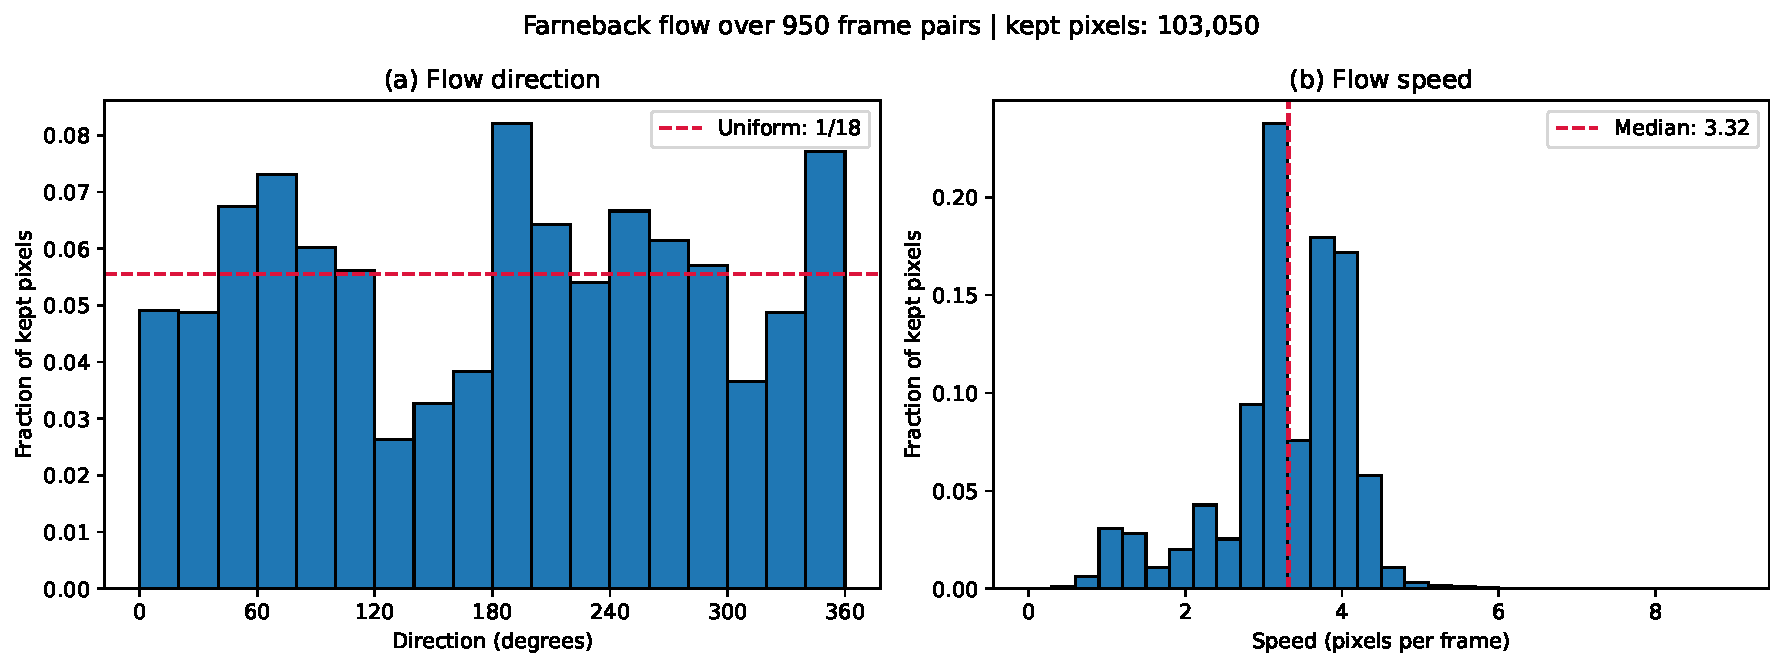
\includegraphics[width=\linewidth]{figures/figure_1.pdf}
\caption{Dense Farneback flow on the first 50 training videos and 950 consecutive frame pairs. The analysis keeps 103,050 pixels. Direction uses 18 bins of 20 degrees; the median, 90th, and 99th percentile speeds are 3.32, 4.12, and 4.67 pixels per frame.}
\label{fig:flow}
\end{figure}

\subsection*{Q2.1: Symmetry and speed in the training data}

The direction histogram covers the full circle. Its bins are not exactly uniform, but no direction family is absent: mirroring maps angle $\theta$ to $180^\circ-\theta$, while rotation maps it to $\theta+90^\circ$ modulo $360^\circ$. Both transformations therefore map trajectories into direction families already represented. The 0.026--0.082 spread across bins is also sensitive to sampling because 50 videos contain only about 100 constant-direction digit trajectories. The median flow speed is 3.32 pixels per frame, so typical 2x and 3x displacements are approximately 6.64 and 9.95 pixels per frame.

Optical flow at overlaps can suppress, combine, or misdirect motion because two digits occupy the same pixels. This can change individual bin heights and the speed tail. It is unlikely to reverse the conclusion because 103,050 pixels from 950 frame pairs remain, directions span all 18 bins, and the central speed mass is concentrated near 3--4 pixels per frame.

\subsection*{Q2.2: Transformation effects}

Mirror and rotation preserve straight constant-velocity motion, elastic wall bounces, and the square domain, but they change digit appearance. Rotation changes appearance more strongly because upright digits become sideways. Speed-up preserves the spatial appearance of each sampled frame but changes temporal displacement and bounce timing between observations. These interventions separate appearance sensitivity from unfamiliar motion and from a hard locality limit: mirror and rotation alter appearance without invalidating the motion law, while speed changes the motion statistics without changing the underlying digit identities.

\section{Baseline ConvLSTM}
\label{sec:q2-baseline}

\begin{table}[htbp]
\centering
\caption{Baseline test performance. Learned-model values are mean (seed 0, seed 1).}
\label{tab:baseline}
\footnotesize
\begin{adjustbox}{max width=\linewidth}
\begin{tabular}{lrrrrrrr}
\toprule
Model & MSE1 & MSE2 & MSE3 & MSE4 & MSE5 & \Efive & Parameters \\
\midrule
A & 0.0186 (0.0190, 0.0182) & 0.0215 (0.0222, 0.0209) & 0.0235 (0.0242, 0.0228) & 0.0250 (0.0258, 0.0242) & 0.0265 (0.0273, 0.0258) & 0.0230 (0.0237, 0.0224) & 480,784 \\
Blank & 0.0426 & 0.0426 & 0.0426 & 0.0425 & 0.0425 & 0.0426 & 0 \\
Copy-last & 0.0492 & 0.0604 & 0.0669 & 0.0708 & 0.0732 & 0.0641 & 0 \\
\bottomrule
\end{tabular}
\end{adjustbox}
\end{table}

\begin{figure}[htbp]
\centering
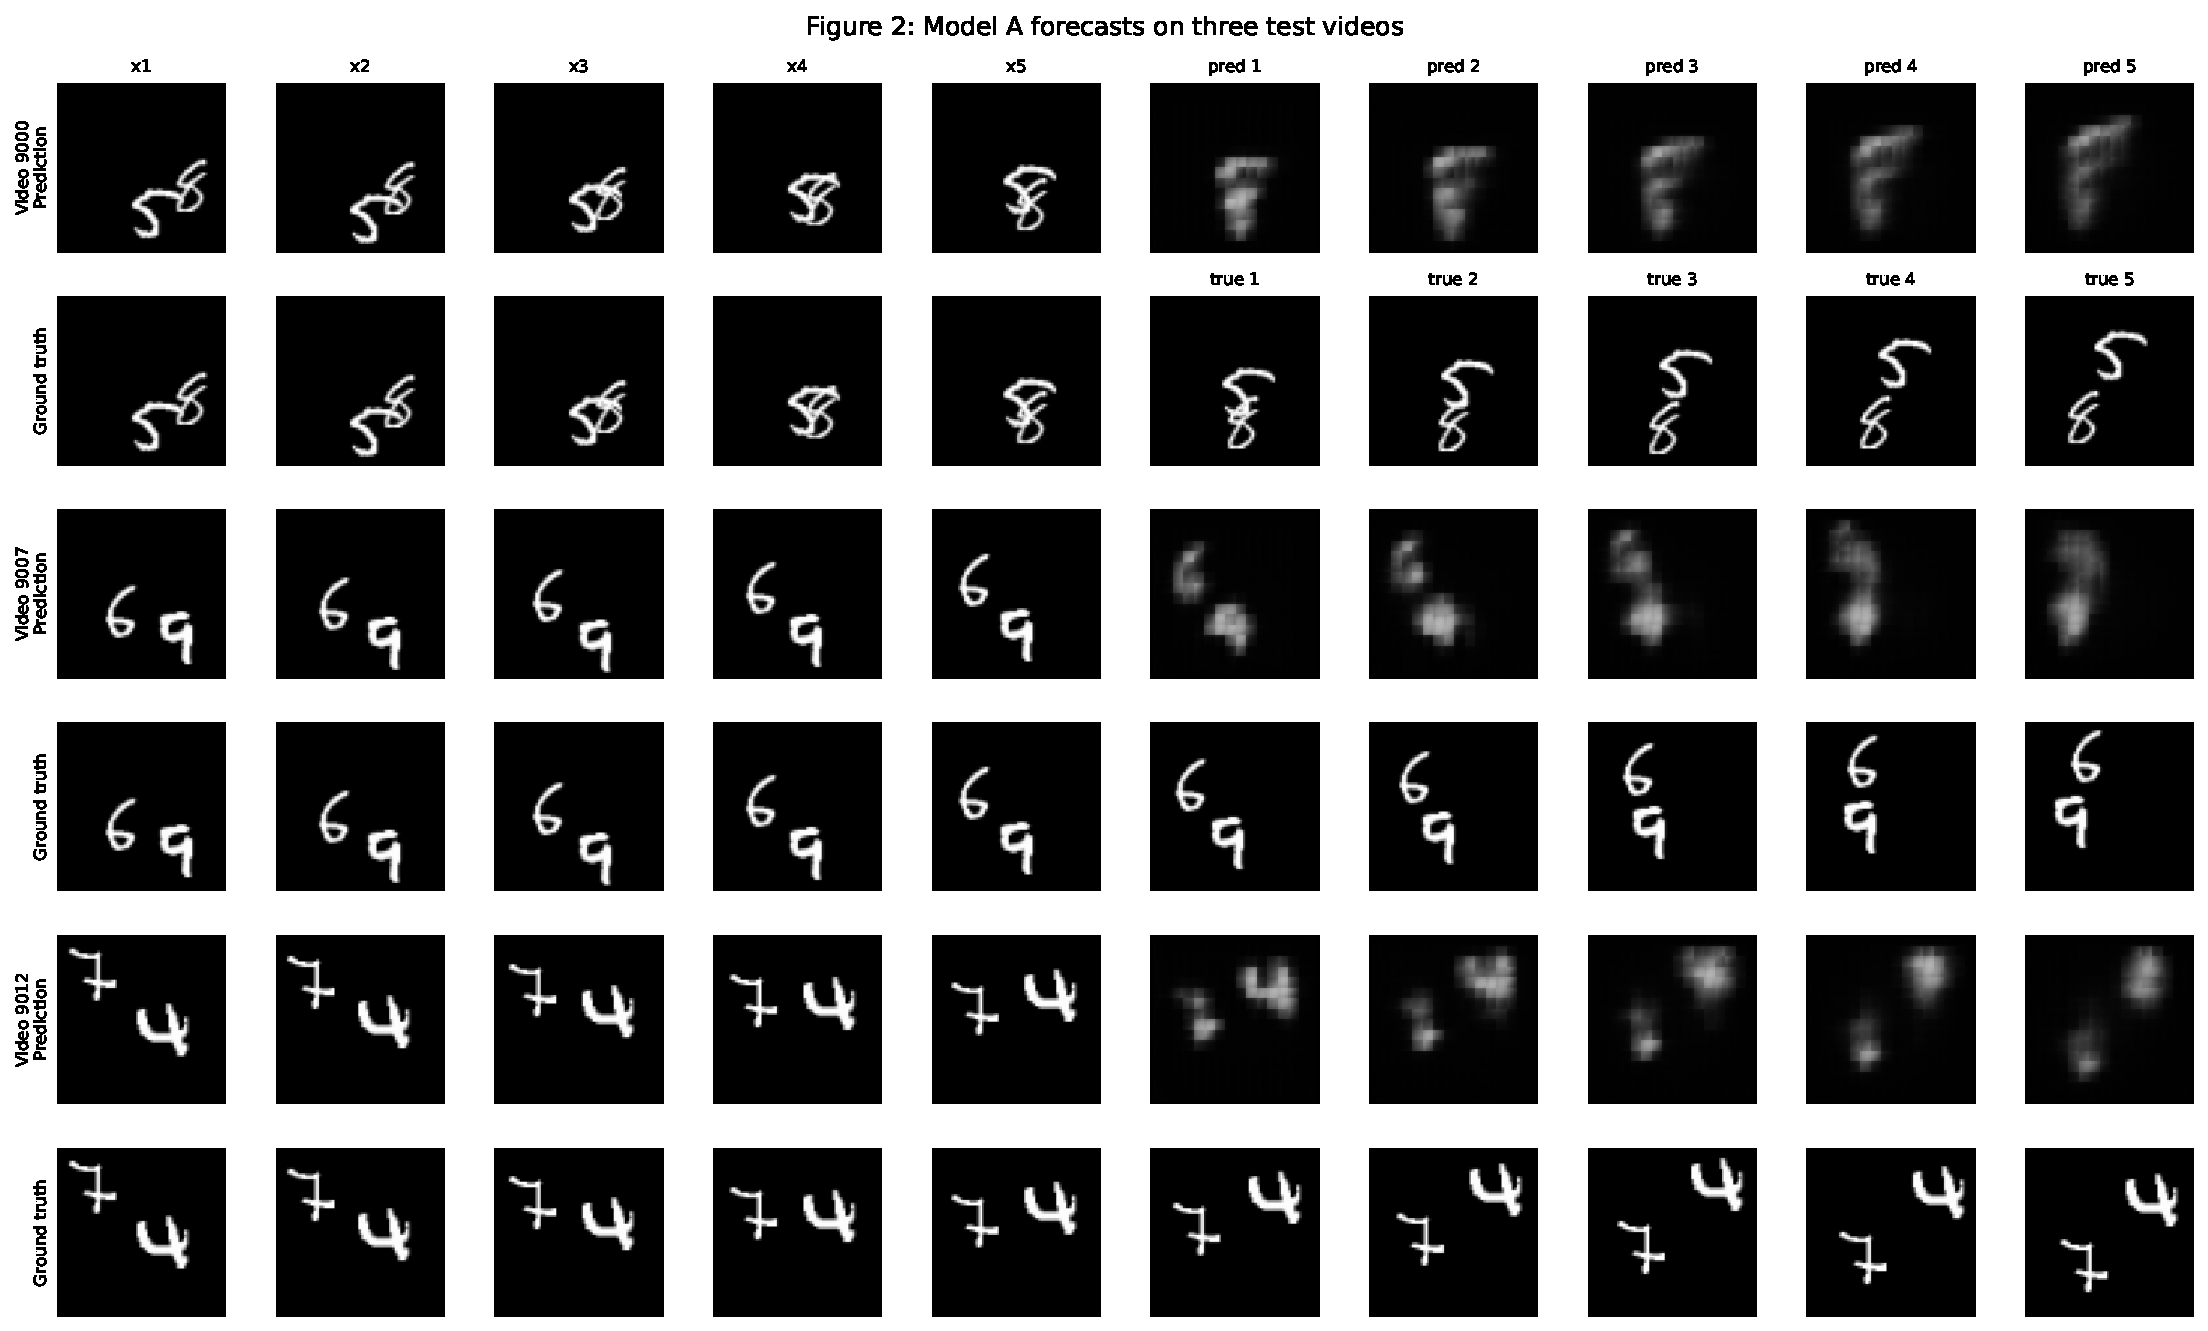
\includegraphics[width=\linewidth]{figures/figure_2.pdf}
\caption{Model A on test videos 9000, 9007, and 9012. Video 9000 contains an overlap in the displayed sequence. Inputs occupy columns 1--5; predictions and ground truth occupy columns 6--10.}
\label{fig:baseline-cases}
\end{figure}

\subsection*{Q2.3: Model A reach}

One cell of the folded $16\times16$ grid corresponds to four original pixels. A $3\times3$ convolution with dilation 1 has radius one folded cell. The longest input-to-output path within one recurrent update passes through the layer-1 gate convolution and then the layer-2 gate convolution, moving at most two folded cells. Paths from the previous hidden states also traverse at most those two convolutions. Cell-state updates are pointwise, while the $1\times1$ output convolution, pixel unshuffle, and pixel shuffle add no reach under the stated convention. Model A's one-step reach is therefore
\begin{equation}
  (1+1)\ \text{folded cells}\times 4\ \text{pixels per cell}=8\ \text{pixels}.
\end{equation}

\subsection*{Q2.4: Baseline performance and overlap behavior}

Model A has \Efive{} 0.0230, compared with 0.0426 for Blank and 0.0641 for Copy-last. It therefore predicts more than a static image prior or persistence. Its error rises monotonically from MSE1 0.0186 to MSE5 0.0265 as autoregressive uncertainty accumulates.

Figure~\ref{fig:baseline-cases} shows that trajectories are followed at 1x, but contours become diffuse across the horizon. During or after overlap, the model tends to merge the two digits into one broad response and does not recover two sharp identities. It preserves approximate motion and occupied region better than precise appearance.

\subsection*{Q2.5: Pre-experiment prediction}

\begin{quote}
\itshape
Before running the mirror, rotation, or speed experiments, I expect model A to be less consistent after both image transformations, with rotation causing the larger failure because it changes digit appearance more strongly even though the transformed motion remains physically valid. The one-step reach is 8 original pixels, so I expect normal-speed prediction to remain usable, 2x motion to degrade, and 3x motion to fail once the displacement between observed frames exceeds what the recurrent update can connect.
\end{quote}

\section{Testing the Baseline}
\label{sec:q2-tests}

\begin{table}[htbp]
\centering
\caption{Mirror and rotation consistency. Model A values are mean (seed 0, seed 1). Every consistency gap is paired with its transformed error.}
\label{tab:consistency}
\footnotesize
\begin{adjustbox}{max width=\linewidth}
\begin{tabular}{lrrrrr}
\toprule
Model & \Efive & \CM & \EM & \CR & \ER \\
\midrule
A & 0.0230 (0.0237, 0.0224) & 0.00199 (0.00143, 0.00255) & 0.0237 (0.0241, 0.0232) & 0.00332 (0.00277, 0.00387) & 0.0247 (0.0251, 0.0244) \\
Blank & 0.0426 & 0 & 0.0426 & 0 & 0.0426 \\
Copy-last & 0.0641 & 0 & 0.0641 & 0 & 0.0641 \\
\bottomrule
\end{tabular}
\end{adjustbox}
\end{table}

The four full worst-case transformation panels are collected as Figure~\ref{fig:transform-cases} in Appendix~\ref{app:qualitative}. They remain part of the report but no longer interrupt the main experimental argument.

\setcounter{figure}{3}
\begin{figure}[htbp]
\centering
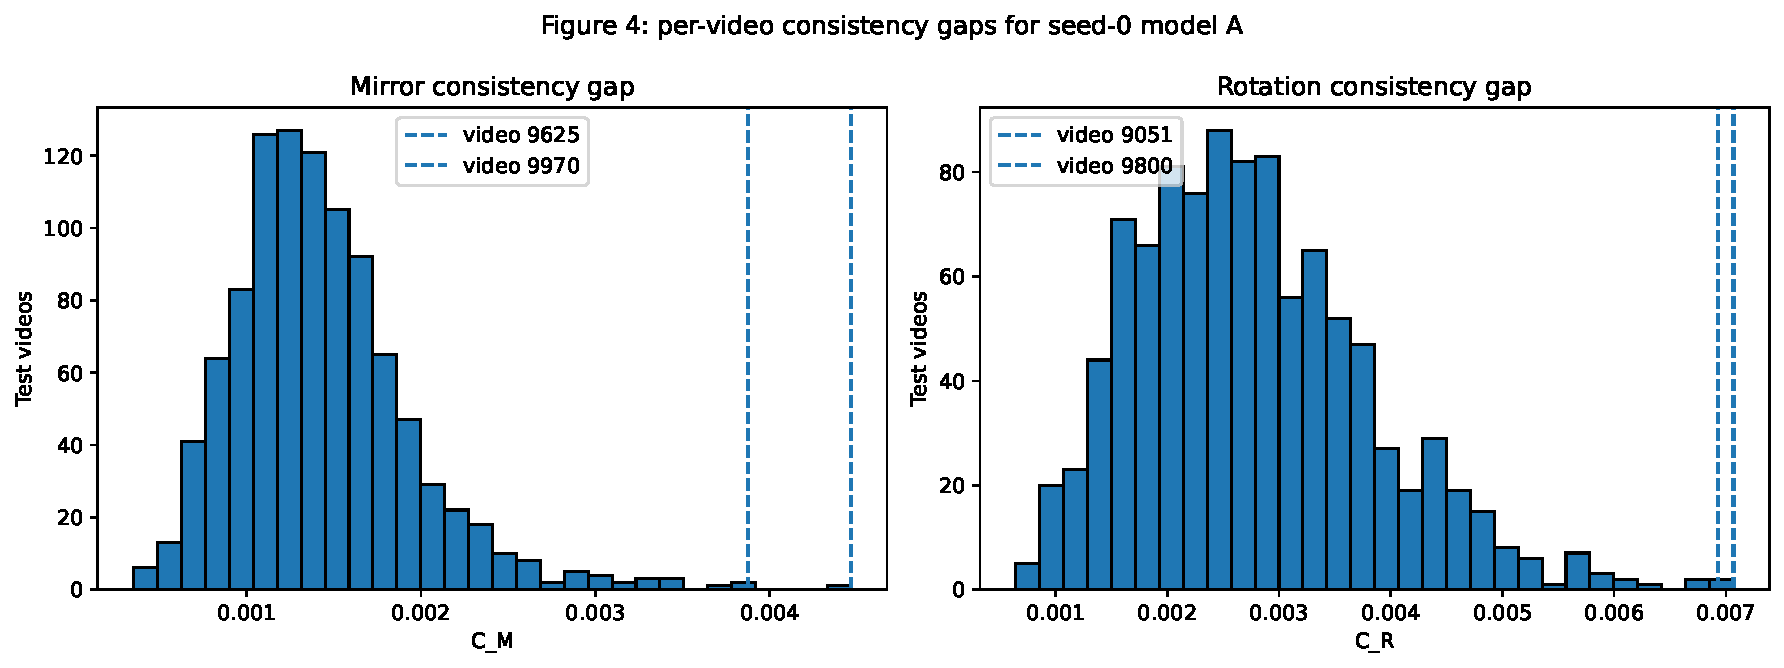
\includegraphics[width=\linewidth]{figures/figure_4.pdf}
\caption{Per-video mirror and rotation consistency gaps for seed-0 model A. Dashed lines mark the four cases in Figure~\ref{fig:transform-cases}.}
\label{fig:gap-histograms}
\end{figure}

\subsection*{Q2.6: Why consistency is insufficient}

Blank and Copy-last have \CM{} and \CR{} exactly zero because zero images and repeated last frames commute with mirror and rotation. Their transformed errors remain 0.0426 and 0.0641. A zero consistency gap therefore proves only that the rule behaves the same after transformation; it does not prove that the rule predicts the future. Every $C_T$ must be read beside $E_T$.

\subsection*{Q2.7: A changed account of motion}

Rotation video 9051 gives the largest seed-0 \CR. In row 3, the forecast from the rotated input begins as a horizontal response but becomes a vertical blob on the left by horizons 4--5, resembling the upright smear produced for the unrotated input in row 1. Row 4 remains horizontal and drifts upward. Neither forecast separates the two digits as the truth does. This is direct evidence that familiar upright appearance affects the predicted motion account. The inputs already contain overlapping digits, so appearance and overlap are confounded in this worst case; the figure supports appearance sensitivity but does not isolate it from overlap.

\subsection*{Q2.8: Rotation versus mirror}

Rotation is harder. Model A has mean \CR{} 0.00332 and \ER{} 0.0247, compared with \CM{} 0.00199 and \EM{} 0.0237. The training flow already spans mirrored and rotated directions, so the difference is not explained by missing direction families. Rotation changes upright digit appearance more severely than a horizontal mirror, and the larger gap and transformed error support appearance sensitivity rather than a change in the valid motion law.

\begin{table}[htbp]
\centering
\caption{Fast-motion test performance. Model A values are mean (seed 0, seed 1).}
\label{tab:speed}
\footnotesize
\begin{adjustbox}{max width=\linewidth}
\begin{tabular}{lrrrrr}
\toprule
Model & \Etwo{} 1x & \Etwo{} 2x & \Etwo{} 3x & \Efive{} 1x & \Efive{} 2x \\
\midrule
A & 0.0201 (0.0206, 0.0196) & 0.0409 (0.0402, 0.0416) & 0.0459 (0.0444, 0.0475) & 0.0230 (0.0237, 0.0224) & 0.0457 (0.0438, 0.0477) \\
Blank & 0.0426 & 0.0425 & 0.0426 & 0.0426 & 0.0425 \\
Copy-last & 0.0548 & 0.0661 & 0.0703 & 0.0641 & 0.0719 \\
\bottomrule
\end{tabular}
\end{adjustbox}
\end{table}

\begin{figure}[htbp]
\centering
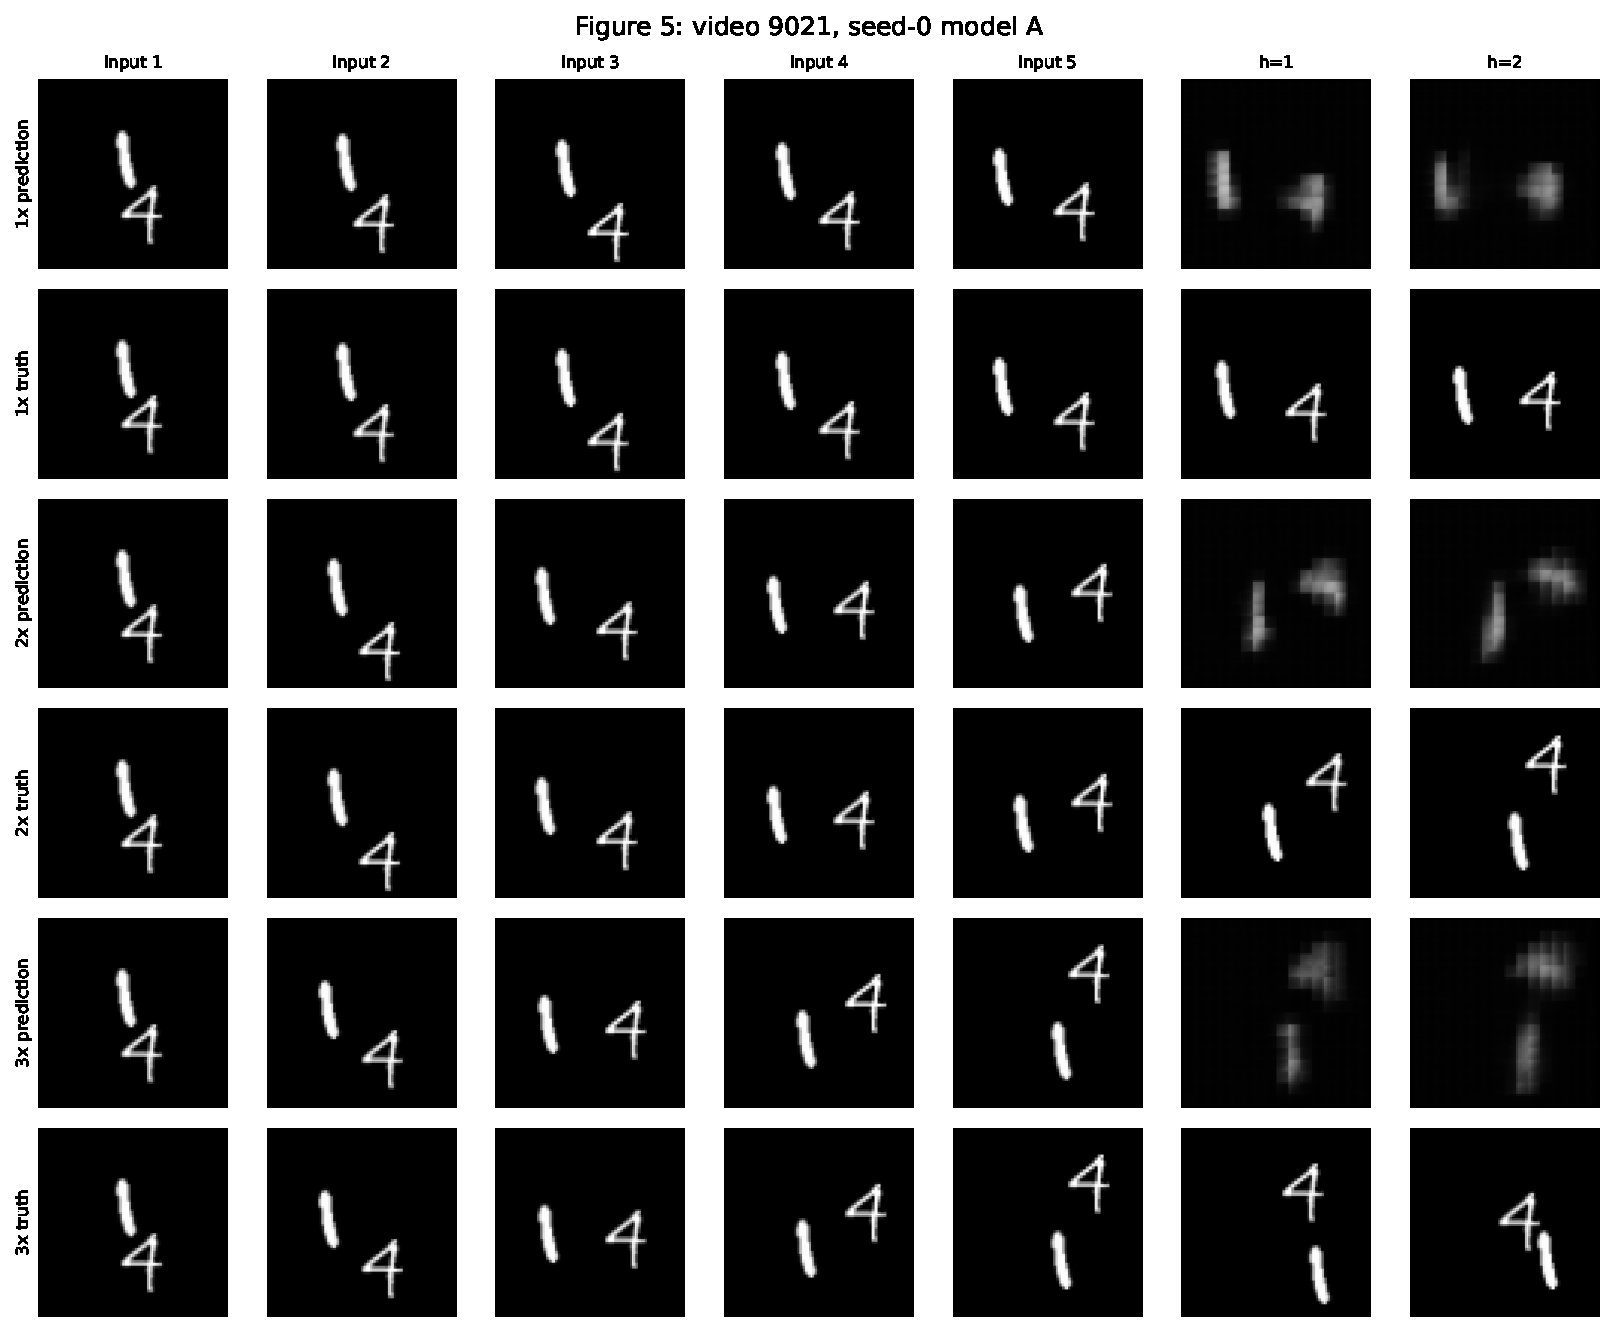
\includegraphics[width=\linewidth]{figures/figure_5.pdf}
\caption{Seed-0 model A on video 9021 at 1x, 2x, and 3x. None of the displayed input or target frames contains overlapping digits.}
\label{fig:speed-case}
\end{figure}
\FloatBarrier

\subsection*{Q2.9: Speed failure}

The failure begins at 2x. Model A's \Etwo{} rises from 0.0201 at 1x to 0.0409 at 2x and 0.0459 at 3x. Its 2x five-horizon error, 0.0457, is already worse than the Blank error 0.0426. At 3x, \Etwo{} also exceeds Blank.

The flow distribution predicts degradation before its median crosses the reach limit. At 2x, 20.3\pct of retained motion pixels exceed model A's 8-pixel reach; at 3x, 83.8\pct exceed it. Reach is only a maximum path length, not a guarantee of tracking, and model A also never observes speed-augmented windows during training. Figure~\ref{fig:speed-case} is interpreted after enforcing no overlap in any displayed input or target frame. At 1x the forecasts blur but follow the pair. At 2x and 3x the predicted objects lag or stall while the true digits continue moving, which is consistent with displacement and exposure failures rather than an overlap-induced merge.

\subsection*{Q2.10: Separating unfamiliar motion and reach}

The baseline results alone cannot distinguish an unseen-speed problem from a reach limit. A sharper diagnostic would generate single-digit clips with controlled displacements from 1 to 16 pixels per frame and train the model-A architecture across the entire sweep. A sharp, persistent error increase near 8 pixels would support a reach limit; a gradual increase removed by training would support unfamiliar motion. Models C and D provide the assignment's coarser available comparison, but D's sparse dilation pattern prevents their difference from isolating reach perfectly.

\section{What Data and Reach Fix}
\label{sec:q2-data}

\subsection*{Q2.11: Pre-experiment prediction}

\begin{quote}
\itshape
I expect model B to reduce the mirror and especially rotation consistency failures, lowering the consistency gaps and transformed errors through symmetry augmentation, while leaving the fast-motion failure largely unchanged. Model C should improve the severe 2x and 3x errors by training on those speeds, but it may still fail at 3x if the 8-pixel one-step reach is the limiting factor. Model D should retain model C's speed adaptation and provide the strongest improvement at 3x because its larger reach can carry information across displacements that model A cannot connect.
\end{quote}

\begin{table}[H]
\centering
\caption{Models A--D on the test split. Values are mean (seed 0, seed 1). All models have 480,784 parameters and were trained on Tesla T4 GPUs.}
\label{tab:models}
\scriptsize
\begin{adjustbox}{max width=\linewidth}
\begin{tabular}{lrrrrr}
\toprule
Model & \Efive{} 1x & \CM & \EM & \CR & \ER \\
\midrule
A & 0.0230 (0.0237, 0.0224) & 0.00199 (0.00143, 0.00255) & 0.0237 (0.0241, 0.0232) & 0.00332 (0.00277, 0.00387) & 0.0247 (0.0251, 0.0244) \\
B & 0.0233 (0.0243, 0.0223) & 0.00124 (0.00108, 0.00139) & 0.0233 (0.0243, 0.0222) & 0.00150 (0.00140, 0.00160) & 0.0233 (0.0243, 0.0222) \\
C & 0.0264 (0.0252, 0.0275) & 0.00152 (0.00200, 0.00104) & 0.0267 (0.0257, 0.0276) & 0.00277 (0.00316, 0.00238) & 0.0276 (0.0266, 0.0286) \\
D & 0.0289 (0.0295, 0.0283) & $9.08{\times}10^{-4}$ ($7.62{\times}10^{-4}$, 0.00105) & 0.0291 (0.0297, 0.0286) & 0.00179 (0.00168, 0.00190) & 0.0298 (0.0304, 0.0293) \\
\bottomrule
\end{tabular}
\end{adjustbox}

\vspace{5pt}
\begin{adjustbox}{max width=\linewidth}
\begin{tabular}{lrrrrrrr}
\toprule
Model & \Etwo{} 1x & \Etwo{} 2x & \Etwo{} 3x & Parameters & Train/epoch (s) & Inference (s) \\
\midrule
A & 0.0201 (0.0206, 0.0196) & 0.0409 (0.0402, 0.0416) & 0.0459 (0.0444, 0.0475) & 480,784 & 10.4 (10.4, 10.4) & 0.327 (0.328, 0.327) \\
B & 0.0201 (0.0213, 0.0189) & 0.0428 (0.0430, 0.0427) & 0.0486 (0.0503, 0.0470) & 480,784 & 10.4 (10.3, 10.4) & 0.323 (0.323, 0.323) \\
C & 0.0231 (0.0221, 0.0241) & 0.0287 (0.0277, 0.0296) & 0.0333 (0.0329, 0.0337) & 480,784 & 9.69 (9.68, 9.70) & 0.329 (0.328, 0.331) \\
D & 0.0267 (0.0272, 0.0261) & 0.0293 (0.0298, 0.0289) & 0.0318 (0.0322, 0.0313) & 480,784 & 9.67 (9.60, 9.74) & 0.327 (0.332, 0.323) \\
\bottomrule
\end{tabular}
\end{adjustbox}
\end{table}

\subsection*{Q2.12: Model D design and reach}

Model D changes only dilation. Both ConvLSTM gate convolutions remain $3\times3$ with 64 hidden channels, but dilation increases from 1 to 2 with padding 2. Input/output shape, parameter count, recurrent rollout, training speeds, loss, and optimisation are otherwise identical to model C. Dilation changes spatial offsets without adding weights, so D retains 480,784 parameters, below the 721,176 limit.

A dilated $3\times3$ convolution has radius two folded cells. The longest path crosses both recurrent layers, giving four folded cells. The one-step reach is
\begin{equation}
  (2+2)\ \text{folded cells}\times4\ \text{pixels per cell}=16\ \text{pixels},
\end{equation}
strictly larger than model A's 8 pixels. This is a nominal maximum, not dense coverage. Dilation 2 preserves row and column parity on the folded grid, so the recurrent computation separates into four interleaved $8\times8$ lattices. Adjacent folded cells cannot exchange state directly. D therefore combines longer paths with missing short-offset connections, and C-to-D differences cannot be attributed to reach alone.

\subsection*{Q2.13: Appearance, unfamiliar motion, and reach}

The mirror and rotation failures are primarily appearance failures. Model B changes only symmetry exposure. Relative to A, it lowers \CM{} from 0.00199 to 0.00124 and \CR{} from 0.00332 to 0.00150; \EM{} and \ER{} both become 0.0233. Since motion directions were already broadly represented, the result supports sensitivity to transformed digit appearance.

The 2x failure is mainly unfamiliar motion. Model C changes only the training-speed distribution and lowers 2x \Etwo{} from 0.0409 to 0.0287. Model D gives 0.0293, no improvement over C at 2x. Exposure accounts for the controlled A-to-C gain, while D's parity split prevents a clean reach-only comparison.

The 3x failure is mixed. Speed augmentation lowers \Etwo{} from 0.0459 for A to 0.0333 for C, so unfamiliar motion explains most of the failure. D reaches 0.0318, a smaller 4.5\pct improvement over C, and only 0.225\pct of 3x retained flow exceeds its nominal 16-pixel radius. The result is compatible with some benefit from longer paths, but it is not clean evidence for a hard reach limit because dilation simultaneously removes adjacent-lattice connections and the seed variation is comparable to the C-to-D difference.

\subsection*{Q2.14: Cost on original clips}

Every speed-robust model loses some 1x accuracy. B is almost unchanged: \Efive{} rises from 0.0230 to 0.0233. C rises to 0.0264, a 14.8\pct increase, while D rises to 0.0289, a 25.7\pct increase. In exchange, D lowers 3x \Etwo{} by 30.7\pct relative to A. Part of D's additional 1x cost may come from its disconnected parity lattices rather than longer reach itself. The trade is worthwhile only when fast-motion robustness is part of the service objective, and model C is preferable if 2x performance and smaller 1x cost matter more than the best measured 3x result.

\section{Final Model}
\label{sec:q2-final}

For any $h\in G$, the symmetrised forecaster is exactly equivariant:
\begin{align}
 \bar f(hX)
 &=\frac{1}{8}\sum_{g\in G}g^{-1}f(ghX) \\
 &=\frac{1}{8}\sum_{k\in G}h\,k^{-1}f(kX)
 =h\,\bar f(X),
\end{align}
where $k=gh$ permutes the eight group elements. Therefore $\bar f(MX)=M\bar f(X)$ and $\bar f(RX)=R\bar f(X)$, making \CM{} and \CR{} zero in exact arithmetic. The measured values are on the order of $10^{-17}$.

\begin{table}[H]
\centering
\caption{Symmetrised models on the test split. Values are mean (seed 0, seed 1).}
\label{tab:symmetrised}
\scriptsize
\begin{adjustbox}{max width=\linewidth}
\begin{tabular}{lrrrrr}
\toprule
Model & \Efive{} 1x & \CM & \EM & \CR & \ER \\
\midrule
Symmetrised B & 0.0227 (0.0237, 0.0216) & $7.91{\times}10^{-17}$ ($7.22{\times}10^{-17}$, $8.60{\times}10^{-17}$) & 0.0227 (0.0237, 0.0216) & $6.47{\times}10^{-17}$ ($5.90{\times}10^{-17}$, $7.03{\times}10^{-17}$) & 0.0227 (0.0237, 0.0216) \\
Symmetrised D & 0.0288 (0.0294, 0.0282) & $5.49{\times}10^{-17}$ ($5.00{\times}10^{-17}$, $5.98{\times}10^{-17}$) & 0.0288 (0.0294, 0.0282) & $4.26{\times}10^{-17}$ ($3.83{\times}10^{-17}$, $4.69{\times}10^{-17}$) & 0.0288 (0.0294, 0.0282) \\
\bottomrule
\end{tabular}
\end{adjustbox}

\vspace{5pt}
\begin{adjustbox}{max width=\linewidth}
\begin{tabular}{lrrrrrrr}
\toprule
Model & \Etwo{} 1x & \Etwo{} 2x & \Etwo{} 3x & Parameters & Train/epoch (s) & Inference (s) \\
\midrule
Symmetrised B & 0.0196 (0.0209, 0.0184) & 0.0419 (0.0423, 0.0416) & 0.0476 (0.0496, 0.0456) & 480,784 & 10.4 (10.3, 10.4) & 2.44 (2.44, 2.44) \\
Symmetrised D & 0.0267 (0.0272, 0.0261) & 0.0292 (0.0297, 0.0288) & 0.0316 (0.0321, 0.0310) & 480,784 & 9.67 (9.60, 9.74) & 2.49 (2.48, 2.49) \\
\bottomrule
\end{tabular}
\end{adjustbox}
\end{table}

The complete final-model transformation and speed panels appear as Figure~\ref{fig:final-transform} in Appendix~\ref{app:qualitative}.

\subsection*{Q2.15: Learned versus built-in symmetry}

Model B learns an approximation to symmetry. Its \CM{} 0.00124 and \CR{} 0.00150 improve on A but remain nonzero. Symmetrisation is exact because group averaging algebraically forces equivariance for any base forecaster. Symmetrised B has \CM{} $7.91\times10^{-17}$ and \CR{} $6.47\times10^{-17}$, while symmetrised D has $5.49\times10^{-17}$ and $4.26\times10^{-17}$. The equality \EM{}$=\ER{}=\Efive{}$ for each symmetrised model is an independent numerical check of the proof.

The exact property costs inference. After three warm-up batches, five sequential full-test timings on an RTX 4050 Laptop GPU give 0.323 seconds for B and 2.44 seconds for symmetrised B, and 0.327 seconds for D and 2.49 seconds for symmetrised D. The roughly 7.6-fold cost matches the eight transformed evaluations up to batching and kernel effects. Training time is unchanged because the wrapper requires no retraining. Averaging can blur when transformed predictions disagree in position or shape, because their inverses form multiple modes. It does not hurt aggregate accuracy here: \Efive{} improves from 0.0233 to 0.0227 for B and from 0.0289 to 0.0288 for D. The final images remain blurry because the underlying forecasts are blurry, not because consistency is inexact.

\subsection*{Q2.16: Revisiting rotation video 9051}

The final model fixes the inconsistency but not the forecast. In Figure~\ref{fig:final-transform}, rows 3 and 4 for video 9051 coincide, so rotating before or after forecasting gives the same result. This part is fixed by group averaging, not by additional training. The predicted future is still a diffuse horizontal response and does not reconstruct the two sharp digits in $T(Y)$. Speed augmentation and larger reach target displacement, but this 1x case is dominated by appearance and forecast sharpness. The final model therefore gives a consistent wrong answer rather than a fully correct one.

\subsection*{Q2.17: Final verdict}

The final model learned a useful but incomplete motion rule. Model A beats Blank and Copy-last, model C handles 2x and 3x after training on those speeds, and model D records a smaller additional 3x improvement despite its sparse dilation pattern. Exact mirror and rotation consistency is supplied by group averaging rather than learned by D. A skeptic should be shown the full A/B/C/D comparison on both seeds, especially the A-to-C speed gain and the uncertain interpretation of the smaller C-to-D difference, together with transformed errors rather than consistency alone. The model still has not passed a non-constant-motion test: acceleration, abrupt direction change, or interacting objects could break a rule learned only from constant velocity and wall bounces.

The broader synthesis is provided in Appendix~\ref{app:discussion}.

\section{Limitations}

Moving MNIST contains only two digits, constant velocity, elastic wall bounces, and pass-through overlaps. The test split measures interpolation within that generator, not general video understanding. The chosen D design uses dilation 2 in both recurrent layers, creating four interleaved parity lattices; its results conflate longer nominal reach with missing adjacent-cell communication. No alternative dilation was selected after viewing test results. Training times were measured during concurrent T4 workflows and are not isolated throughput. Inference times were remeasured sequentially after warm-up and remain hardware-specific deployment costs.

The river proposal is not empirically validated because no river dataset is supplied. Its main risks are the unmonitored tributary, sparse rainfall coverage, changing travel time, and schedule deviations. Those risks are represented explicitly rather than resolved by architecture alone.

\section{Conclusion}

The river design uses causal alignment, directed connectivity, horizon-relative delay, S1-local release forcing, and calibrated predictive intervals to keep issuance-time information explicit. The Moving MNIST study reaches a parallel conclusion through experiments: data repairs much of unfamiliar motion, receptive pattern matters beyond maximum radius, and symmetry can be guaranteed algebraically without guaranteeing accuracy. Model B improves learned consistency, C produces the main fast-motion gain, D records a smaller but confounded 3x gain, and symmetrised D makes mirror and rotation consistency exact. The resulting forecaster is more robust, but its blur and normal-speed trade-off prevent a claim of complete motion understanding.

\begin{thebibliography}{2}

\bibitem[Shi et~al.(2015)Shi, Chen, Wang, Yeung, Wong, and Woo]{shi2015convlstm}
Xingjian Shi, Zhourong Chen, Hao Wang, Dit-Yan Yeung, Wai-Kin Wong, and Wang-chun Woo.
\newblock Convolutional LSTM network: A machine learning approach for precipitation nowcasting.
\newblock In \emph{Advances in Neural Information Processing Systems}, volume 28, 2015.

\bibitem[Srivastava et~al.(2015)Srivastava, Mansimov, and Salakhutdinov]{srivastava2015moving}
Nitish Srivastava, Elman Mansimov, and Ruslan Salakhutdinov.
\newblock Unsupervised learning of video representations using LSTMs.
\newblock In \emph{International Conference on Machine Learning}, pages 843--852, 2015.

\end{thebibliography}

\clearpage
\appendix
\renewcommand{\theHfigure}{appendix.\arabic{figure}}

\section{Qualitative Evidence}
\label{app:qualitative}

\setcounter{figure}{2}
\begin{figure}[H]
\centering
\begin{subfigure}{\linewidth}
\centering
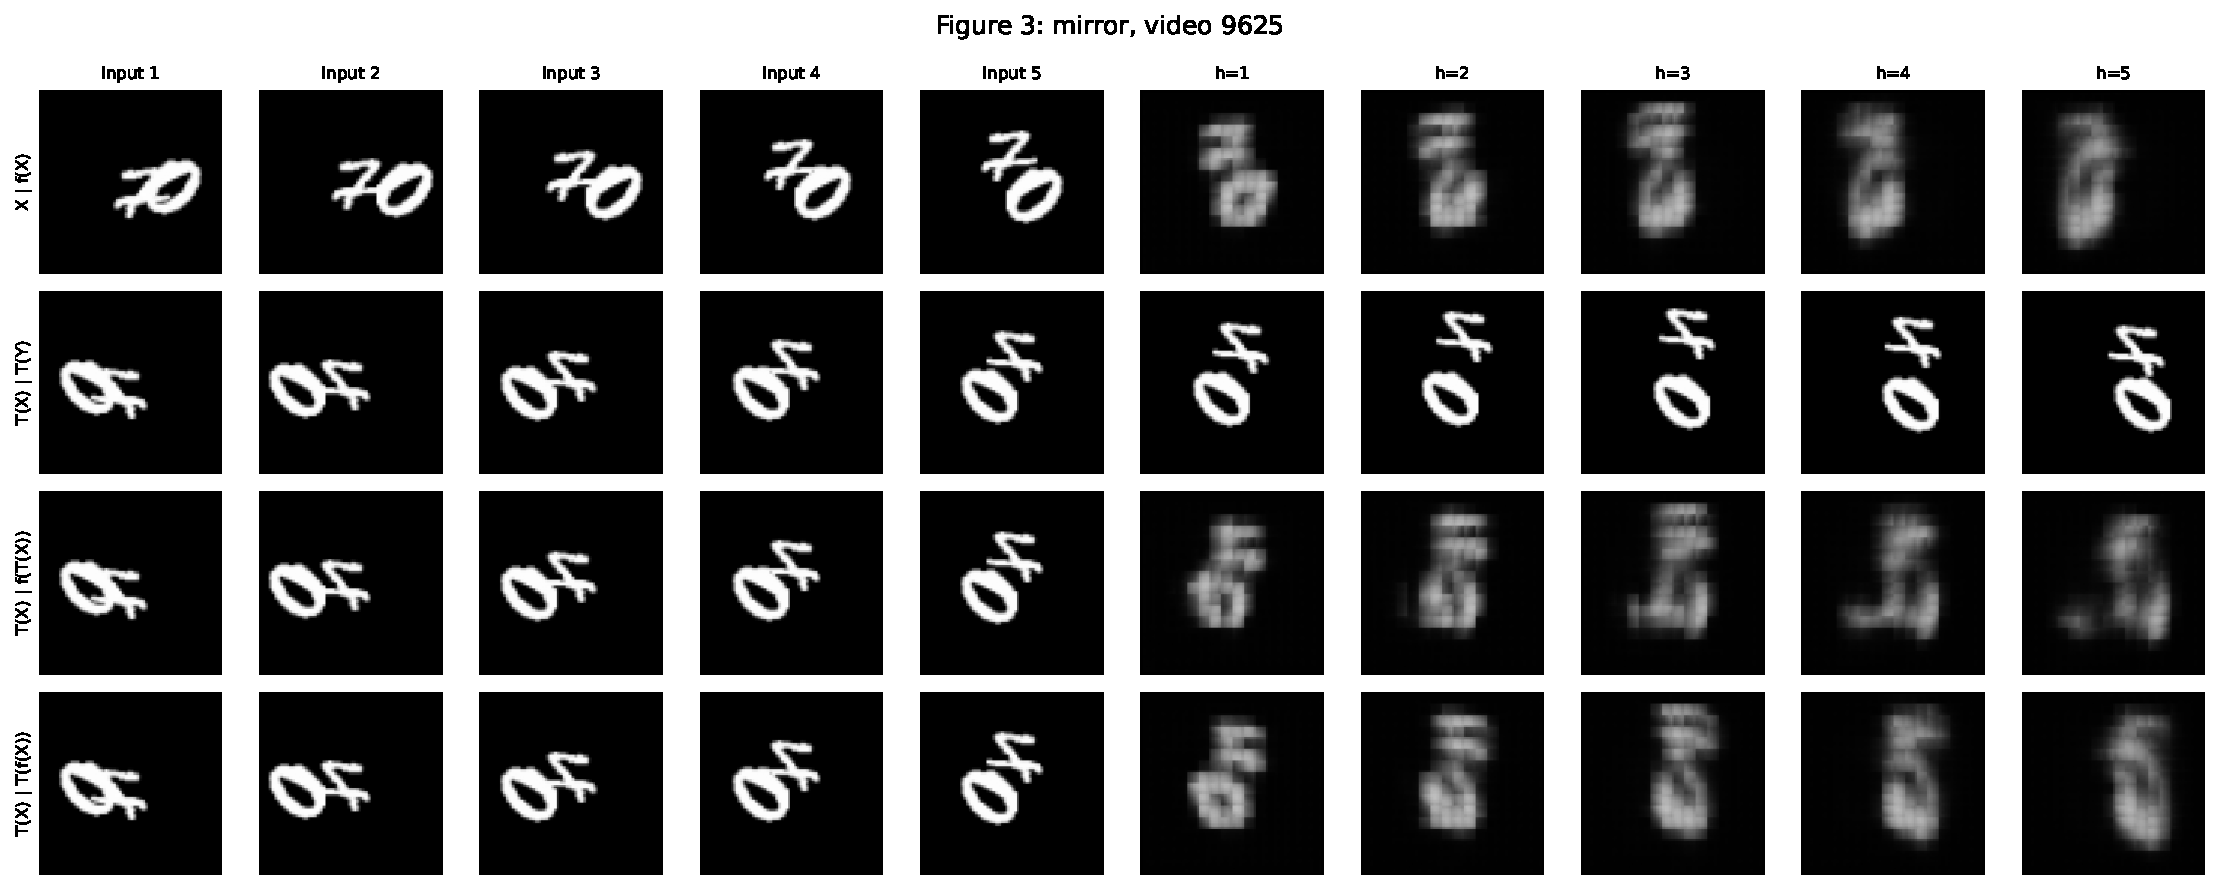
\includegraphics[width=\linewidth]{figures/figure_3_mirror_video_9625.pdf}
\caption{Mirror rank 1, video 9625.}
\end{subfigure}

\begin{subfigure}{\linewidth}
\centering
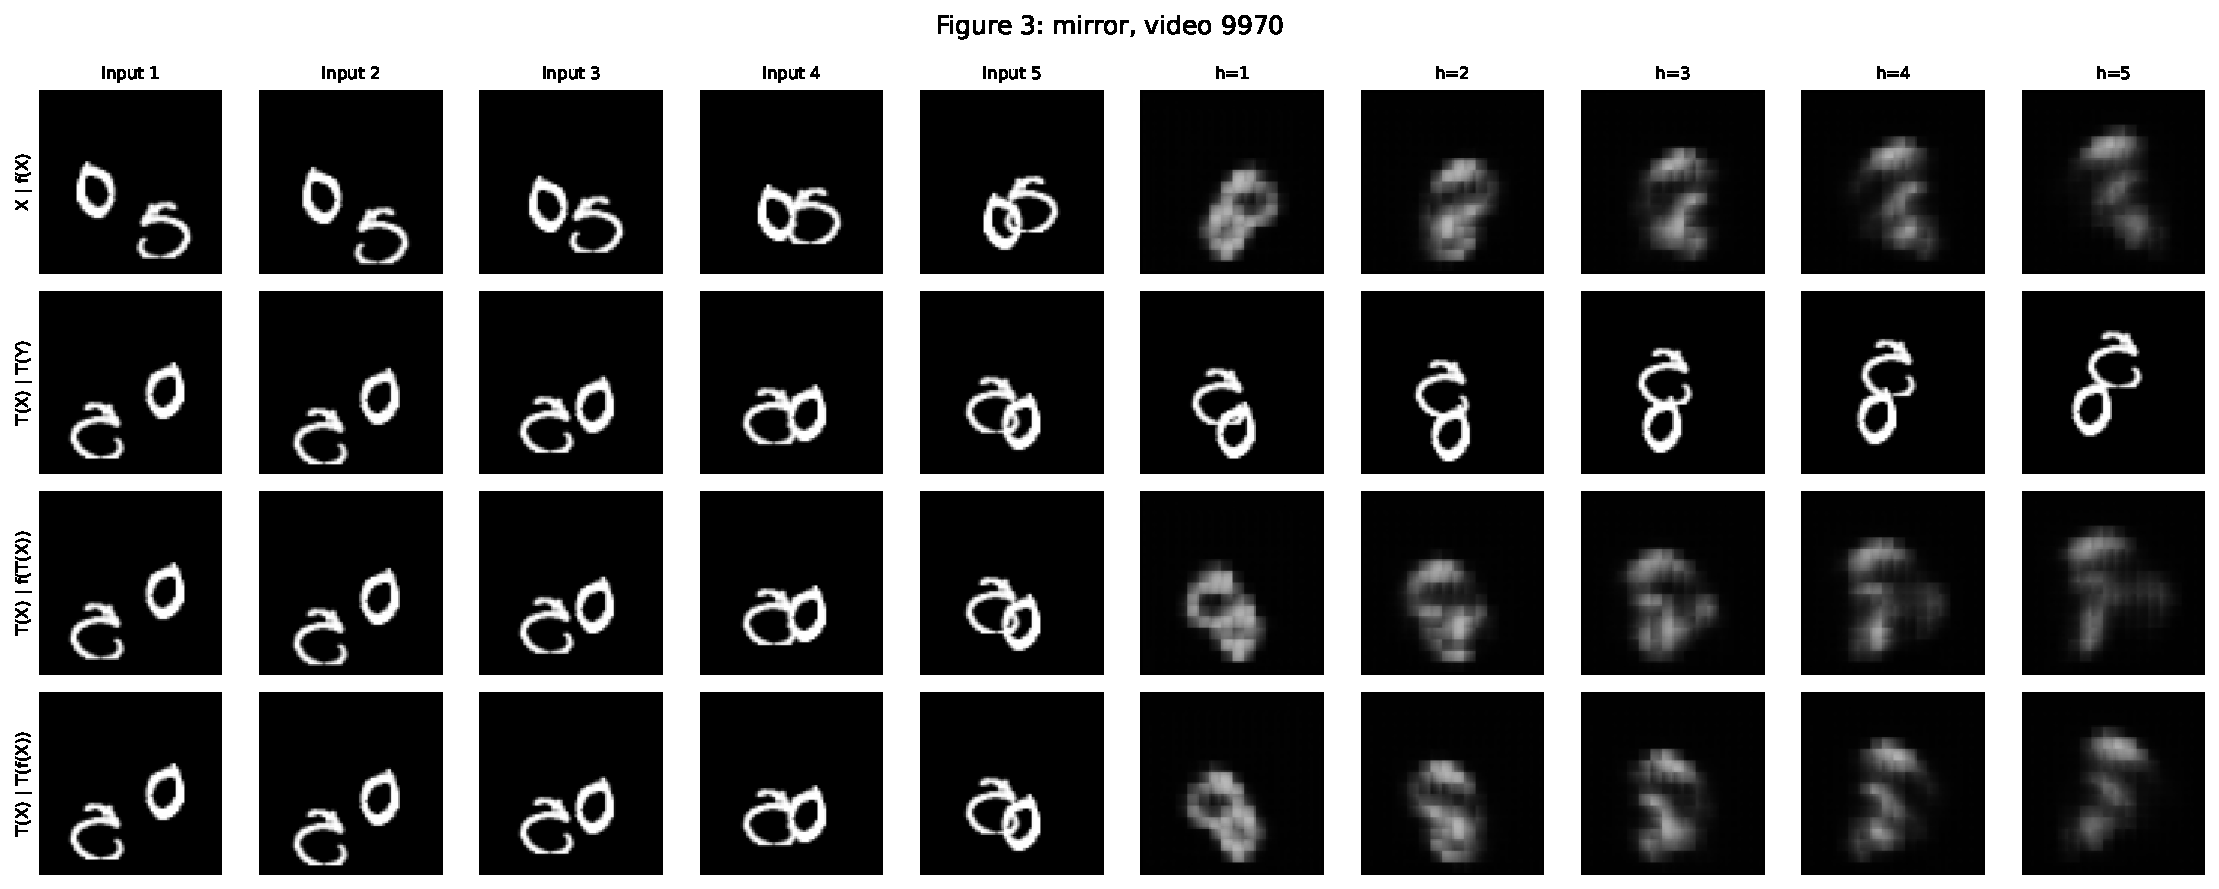
\includegraphics[width=\linewidth]{figures/figure_3_mirror_video_9970.pdf}
\caption{Mirror rank 2, video 9970.}
\end{subfigure}
\caption{Largest seed-0 model A mirror-consistency failures. Each panel shows $X\mid f(X)$, $T(X)\mid T(Y)$, $T(X)\mid f(T(X))$, and $T(X)\mid T(f(X))$. GIFs: \protect\path{artifacts/gifs/figure_3_mirror_video_9625.gif} and \protect\path{artifacts/gifs/figure_3_mirror_video_9970.gif}.}
\label{fig:transform-cases}
\end{figure}

\begin{figure}[H]
\ContinuedFloat
\centering
\begin{subfigure}{\linewidth}
\centering
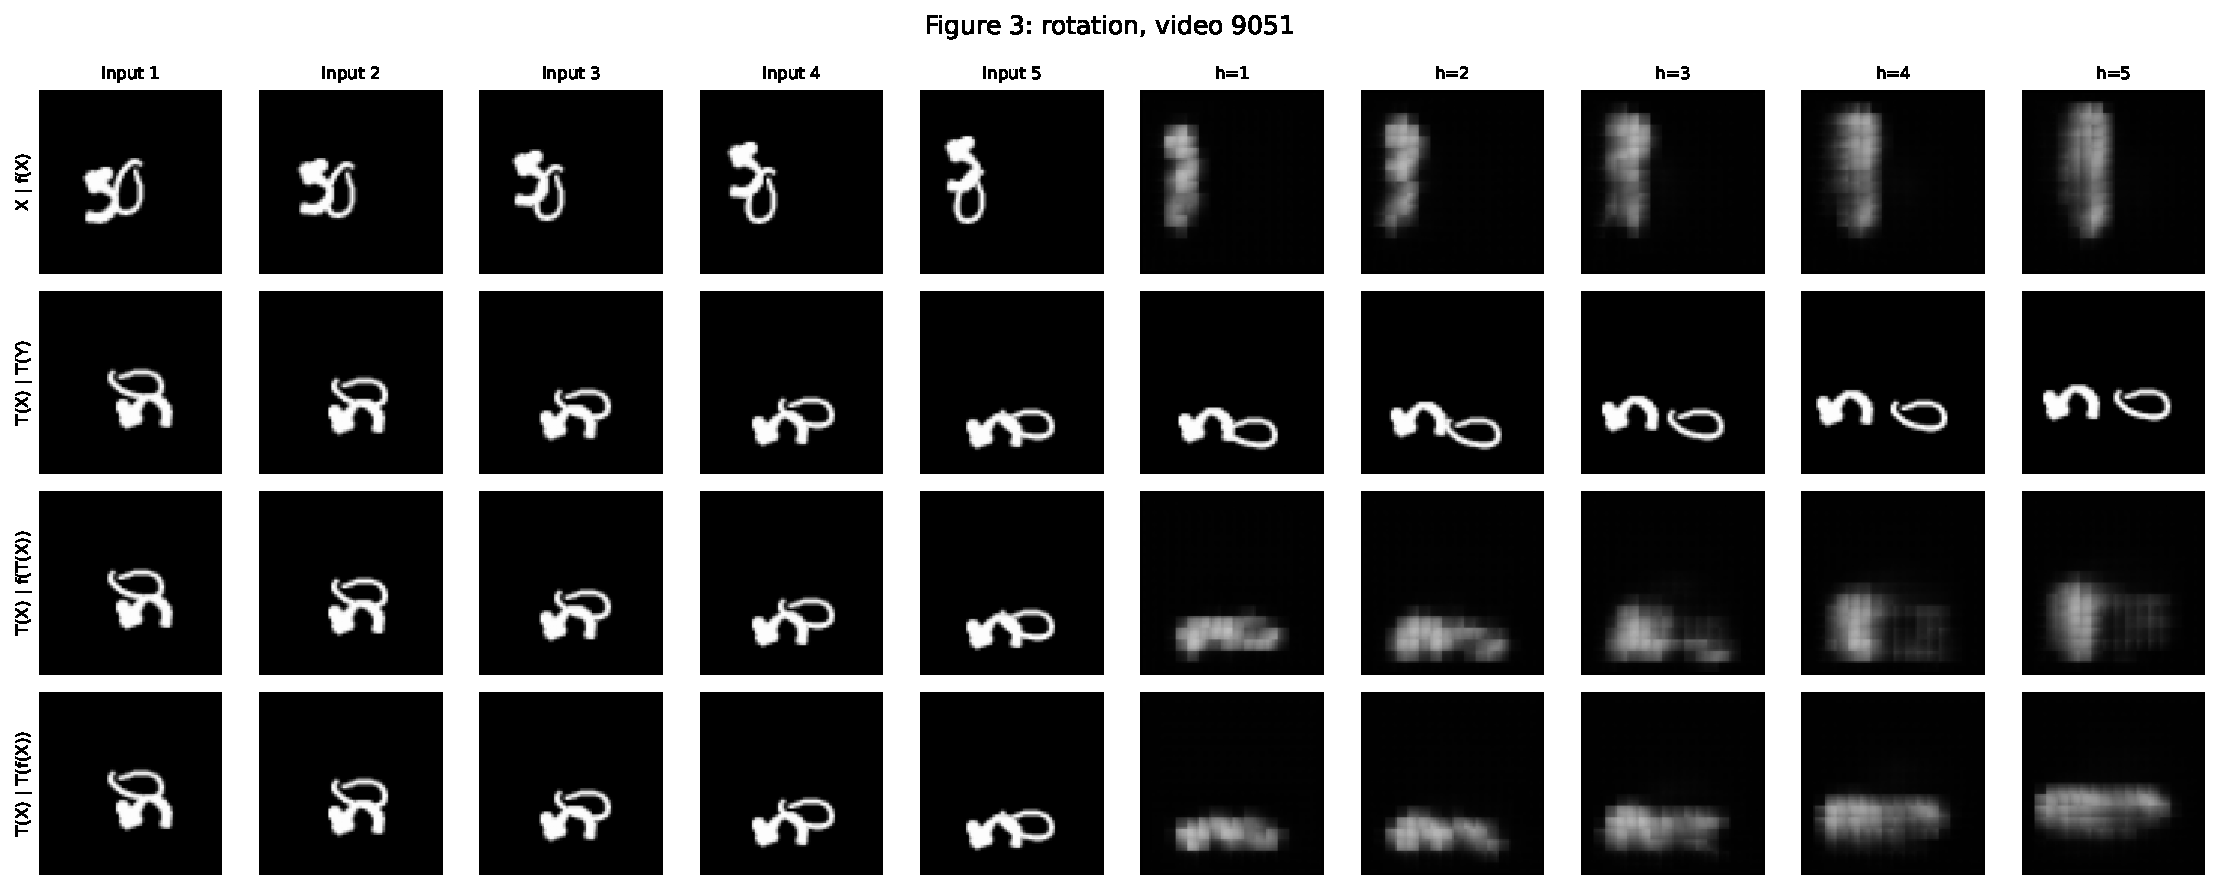
\includegraphics[width=\linewidth]{figures/figure_3_rotation_video_9051.pdf}
\caption{Rotation rank 1, video 9051.}
\end{subfigure}

\begin{subfigure}{\linewidth}
\centering
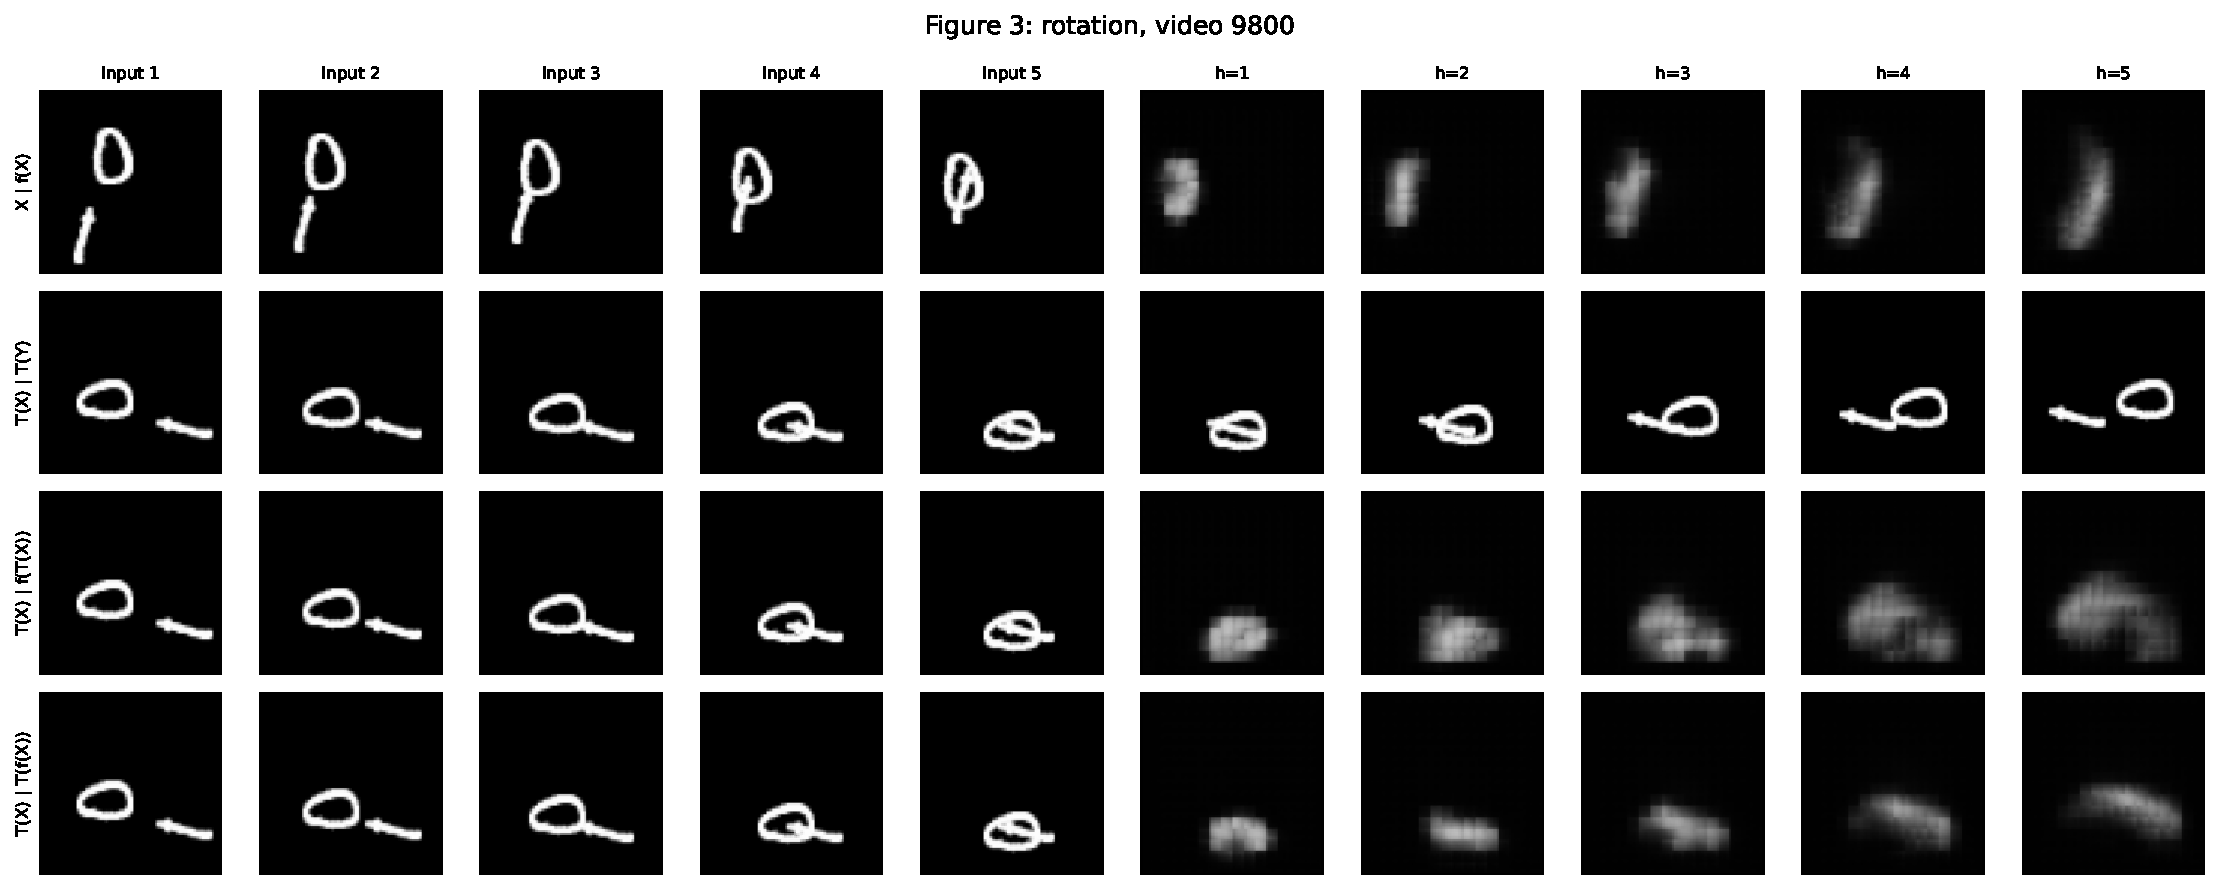
\includegraphics[width=\linewidth]{figures/figure_3_rotation_video_9800.pdf}
\caption{Rotation rank 2, video 9800.}
\end{subfigure}
\caption[]{Largest seed-0 model A rotation-consistency failures (continued). GIFs: \protect\path{artifacts/gifs/figure_3_rotation_video_9051.gif} and \protect\path{artifacts/gifs/figure_3_rotation_video_9800.gif}.}
\end{figure}

\setcounter{figure}{5}
\begin{figure}[H]
\centering
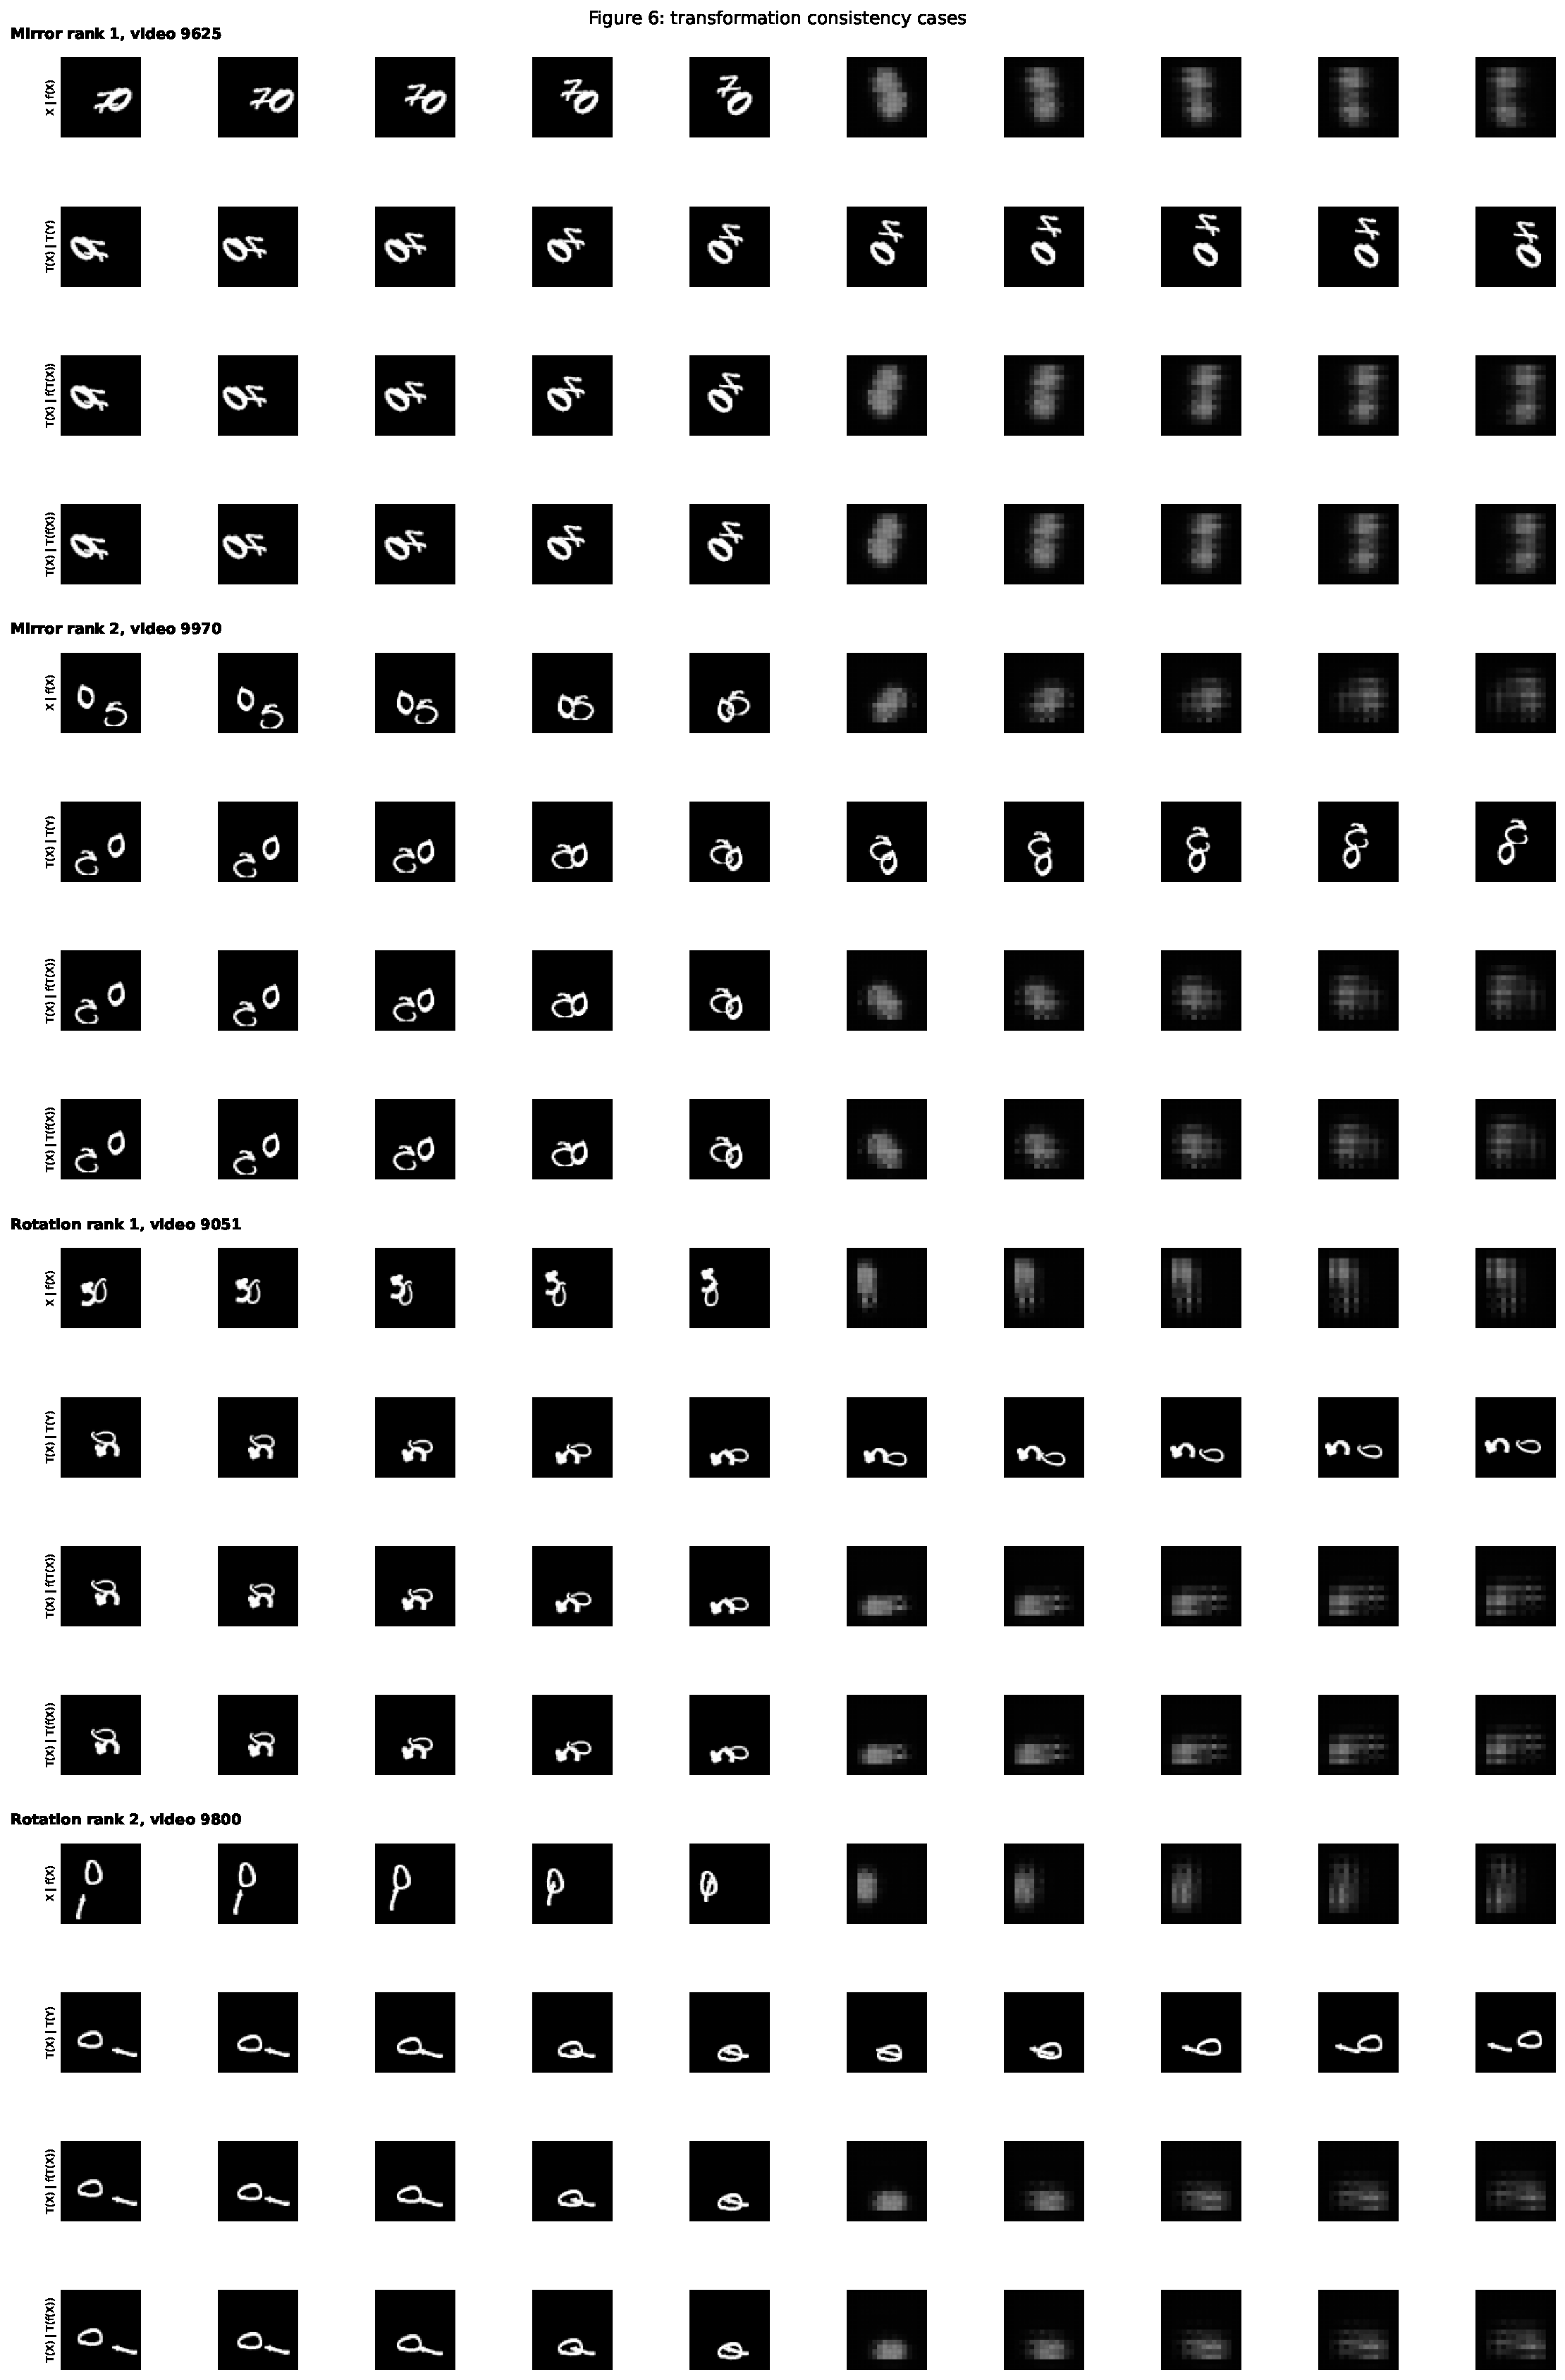
\includegraphics[height=0.82\textheight,keepaspectratio]{figures/figure_6a.pdf}
\caption{Final symmetrised-D transformation cases on exactly the Figure~\ref{fig:transform-cases} videos. Rows 3 and 4 now agree up to floating-point error. GIFs: \protect\path{artifacts/gifs/figure_6_mirror_video_9625.gif}, \protect\path{artifacts/gifs/figure_6_mirror_video_9970.gif}, \protect\path{artifacts/gifs/figure_6_rotation_video_9051.gif}, and \protect\path{artifacts/gifs/figure_6_rotation_video_9800.gif}.}
\label{fig:final-transform}
\end{figure}

\begin{figure}[H]
\ContinuedFloat
\centering
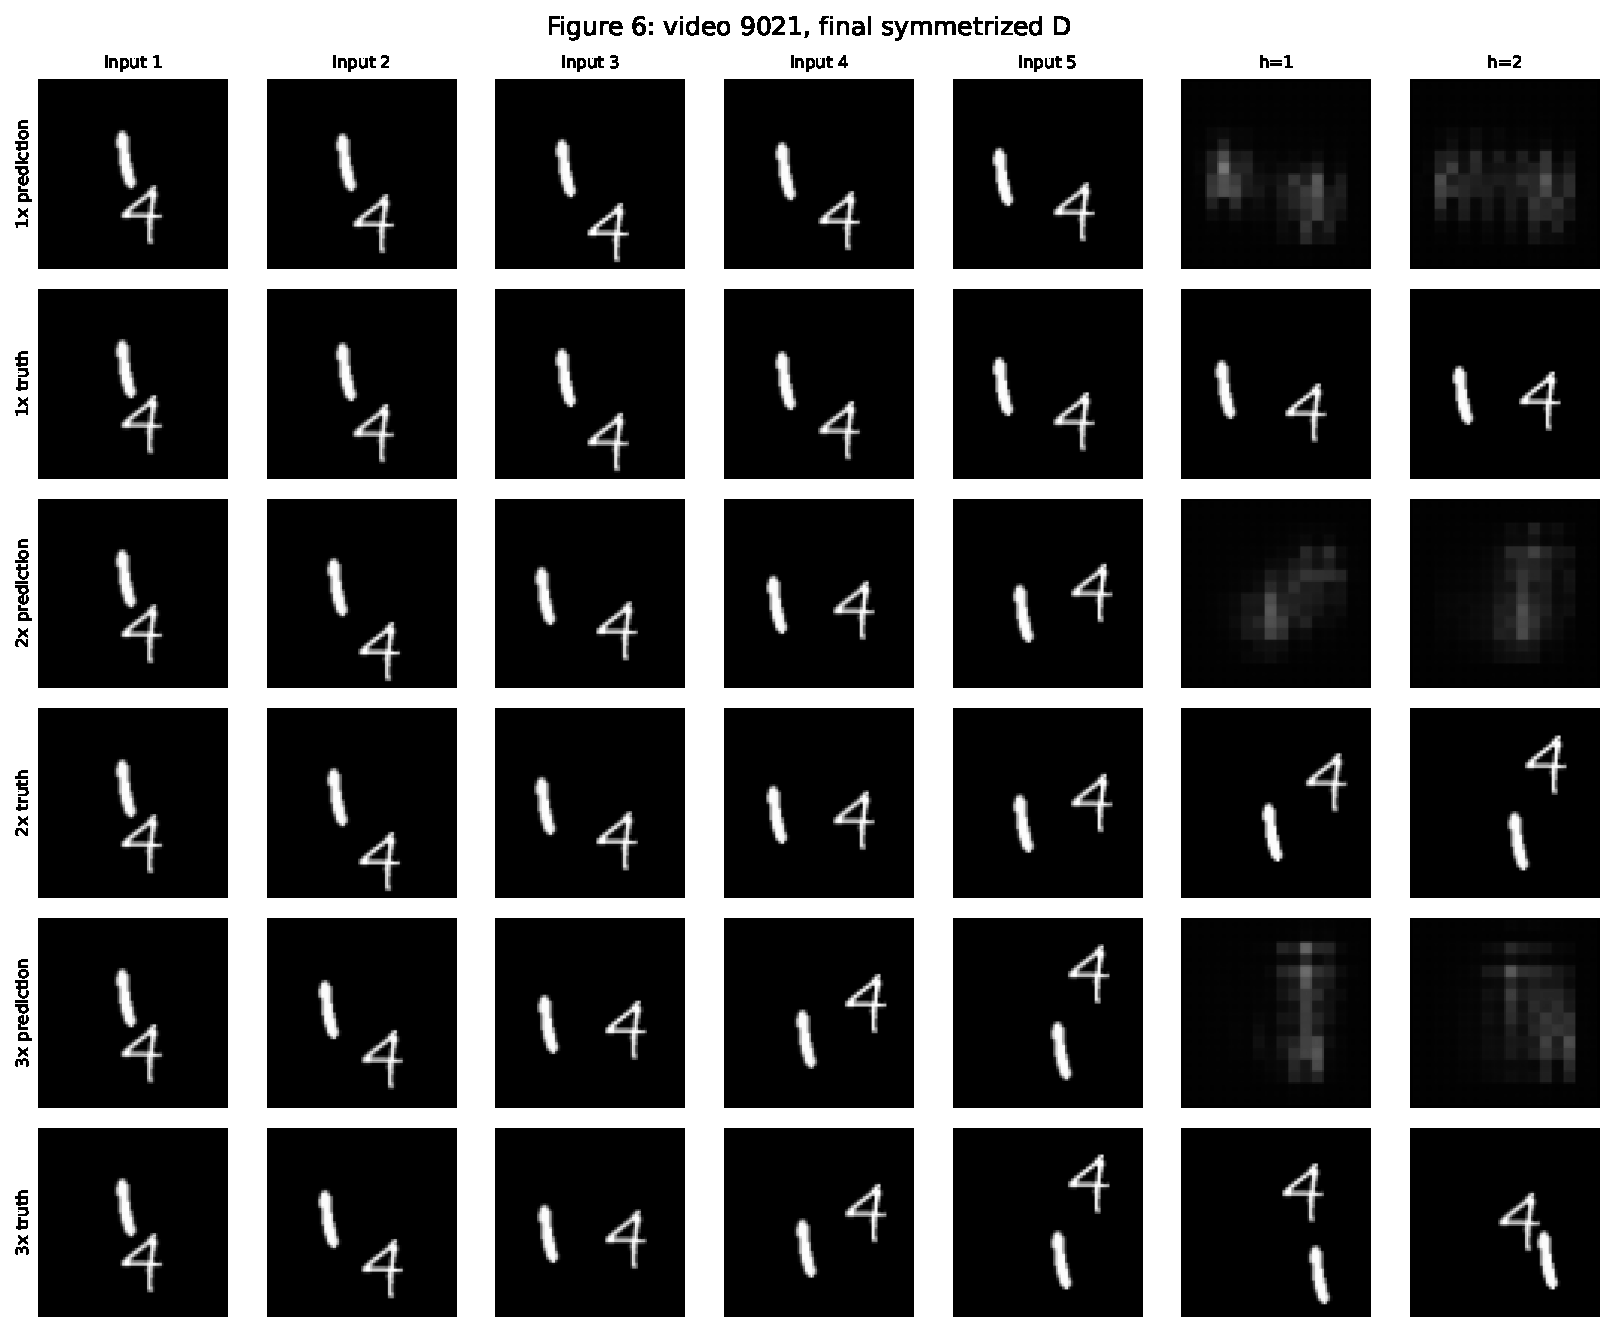
\includegraphics[width=\linewidth]{figures/figure_6b.pdf}
\caption[]{Final symmetrised-D stress tests (continued). The same video 9021 from Figure~\ref{fig:speed-case} is shown at 1x, 2x, and 3x.}
\label{fig:final-speed}
\end{figure}
\FloatBarrier

\section{Discussion}
\label{app:discussion}

The experiments separate three causes that would be confounded in one test. B shows that transformed appearance contributes to mirror and rotation failures. C shows that most fast-motion degradation is repaired by exposure to fast windows. D records a smaller gain only at the largest tested displacement, but its sparse dilation pattern prevents that difference from identifying reach alone. The evidence does not support a single explanation for every failure.

The final model prioritises exact symmetry and 3x robustness over 1x sharpness and inference cost. Symmetrised B is the strongest choice for original-speed accuracy and exact transformation consistency, but it inherits B's poor fast-motion behavior. Symmetrised D is selected because the assignment's final objective includes fast motion and larger reach. Its limitations remain visible: group averaging guarantees a relationship between transformed predictions, not correctness, object identity, or sharpness.

\end{document}
